\documentclass[b5,12pt]{report}
\usepackage{graphicx}
\usepackage{multirow} % used in multi-row table
\usepackage{color} % set color for text
\usepackage[margin=1in]{geometry}  % set margin size
\usepackage[linesnumbered,boxed]{algorithm2e}  % display algorithm
\usepackage{amsmath}
\usepackage{amssymb}
\usepackage{hyperref} % add link for tableofcontents
\linespread{1.5}
\usepackage{anysize}
\marginsize{3cm}{2cm}{1.2cm}{1.2cm} % need package anysize
\setcounter{secnumdepth}{3} % set the section depth
\setcounter{tocdepth}{2}
\title{Tracking the Movement of Microglia Cells and the Growing of Neurons in Zebra Fish Brain}
\begin{document}
\maketitle
\begin{abstract}
 This is cool paper about tracking.
\end{abstract}
\renewcommand{\abstractname}{Acknowledgements}
\begin{abstract}
 Thanks Mum!
\end{abstract}

\tableofcontents
\listoffigures
\part{Thesis overview}
\chapter{Introduction}
\section{Background}
\subsection{Why bioimage informatics matters}
\subsection{Current imaging techniques}
\subsection{The cells in Zebra fish brain}
\section{Motivation and my work}
The movement of microglia cells and the growing of neuron cells.
\section{Thesis organization}
The rest of the thesis is organized as follows. Part 2 describes the cell tracking methods (chapter \ref{chpt:celltracking}) and the related image segmentation (chapter \ref{chpt:imgseg}), component tree construction (chapter \ref{chpt:cptree}) and tree assignment methods (chapter \ref{chpt:treeassign}). Part 3 describes the automatic neuron tracing methods (chapter \ref{chpt:auto-nt}), human guided neuron tracing methods (chapter \ref{chpt:manual-nt}) and the powerful fastmarching method (chapter \ref{chpt:fm}).
\part{Cell Tracking}
\chapter{Image segmentation} \label{chpt:imgseg}
For the cell tracking methods which seperate the segmentation and association steps, the segmentation quality influences the whole tracking result significantly. A good segmentation for the objects in each frame is very important especially in the very early frames. Because the segmentation results of priori frame affects the segmentation results of later frames, that the missing-segmentation of an object will be very likely to be miss tracked in later frames.

Image segmentation are basically ad-hoc problems. Different segmentation emphasize one or more of the desired properites. During the past 40 years, hundreds of segmentation algorithms have been proposed\cite{freixenet2002yet}. Some basic segmentation methods, such as global/local thresholding and some complex segmentation models, such as active contour, chanvese's method , and graph cut method, will be introduced in this chaper.

In this thesis, I proposed a voronoi-diagram based multi-cell segmentation method, which needs only one level set function. It is an extension of Dufour \cite{dufour2005segmenting} and Zhang's method \cite{zhang2004tracking} without considering the coupling constraints (usually unnecessary). The key idea of my method is to build a voronoi diagram for all cells by using fastmarching method. Then each object performs the chanvese's segmentation method in its own voronoi area. I build an image processing platform with lots of image segmentation algorithms in C/C++, which is distributed as an open source repository.
\section{Thresholding method}
\subsection{Overview}
In digital image processing, thresholding is the mostly used technique for image segmentation due to its easy usage. Normally the thresholding value is a single value which partitions a grayscale image into foreground and background area. It is offen an effective tool to separate objects from the background and it is always the first tried method before applying other complex segmentation methods. One application of thresholding is document image analysis which aims to extract printed characters \cite{kamel1993extraction,abak1997performance}, graphs, or other items. Examples of thresholding applications lies in all kinds of pre-processing or post-processing steps, including edge detection, image feature extraction, distance transform, skeleton extraction, cell tracking and so on. In practice, thresholding can solve most problems. However, a good thresholding value is required.

Although its simplicity, there is no strict definition for the thresholding of an image. Quite a lot of thresholding techniques \cite{sahoo1988survey, sankur2001image, sezgin2004survey}, more than 44 binary methods, are proposed according to different criterions. Sezgin and Sankur \cite{sankur2001image, sezgin2004survey} categorize thresholding methods into six groups based on different models, that is histogram shape-based methods, clustering-based methods, entropy-based methods, object attribute-based methods, spatial methods, and local methods. Histogram shape-based methods find the thresholding value on histogram data by seperating the peaks and valleys, the representing method is otsu's thresholding method. Clustering-based methods models the foreground and background as a mixture of two gaussians and applys clustering methods to get the two parts. Entropy-based methods utlize the entropy of the foreground and the background regions, as well as the cross-entropy between the original and binarized image, etc. Object attribute-based methods finds a partition which is similar to the gray-level image in some attributes, such as fuzzy shape similarity, edge coincidence, etc. The spatial methods utilize the probability distribution in higher-order and/or correlation between pixels. Local methods calculate a suitable threshold value for each pixel according to the local image characteristics, such as the standard devariance, mean, etc.

As thresholding method is not the main segmentation method in our paper, we only introduce some widely used algorithms. For global thresholding method, otsu's method \cite{otsu1975threshold} is a very elegant method with solid mathematic fomulars by minimize the intra-class variance or maximize inter-class variance. And it is easy to extend otsu's method into multi-thresholding method. For local thresholding, the thresholding is decided by average local gray values and/or standard devariance. 
\subsection{Global thresholding and Otsu's method}
Global thresholding converts a grey-level image into binary image by turning all pixels below some threshold to zero and all pixels above that threshold to one. If $g(x,y)$ is a thresholded version of $f(x,y)$ at some global threshold $T$, 
\begin{equation}
g(x,y) = \left\{
  \begin{array}{ll}
  1 & \mbox{if } f(x,y) \ge T \\
  0 & \mbox{otherwise}
  \end{array}
  \right.
\end{equation}
To set a global threshold $T$, we usually analysis the histogram profile by finding a valley that seperates two mountains. One mountain for the foreground and one for the background. The histogram of an image is a probability distribution,
\begin{equation}
p(g) = n_g/n
\end{equation}
where, $n_g$ is the number of pixels with intensity $g$, $n$ is the total number of pixels. There are two ways to decide the global threshold, the iterative method and otsu's method. 

\textbf{Iterative method :} This method compute the global threshold from the initial mean intensity value, then iterative replace the threshold value by the average mean intensity of the foreground and the background regions. See alg\ref{alg:global-thresh} for details of this method.

The main problem for the iterative method is speed. The step for segmenting an image into foreground and background for many times is time consuming.

\begin{algorithm}
\SetAlgoLined
\KwData{Grey-level image and the histogram}
\KwResult{The global threshold}
Estimate the initial threshold $T$ with the mean value.\\
Divide the image into foreground area $F$ and background area $B$.\\
Calculate the mean intensity $\mu_f$ and $\mu_b$ for area $F$ and $B$ respectively.\\
Refresh the threshold $T = (\mu_f + \mu_b)/2$\\
Repeat 2-4 until $\mu_f$ and $\mu_b$ do not change any more
\caption{Iterative method for global thresholding}
\label{alg:global-thresh}
\end{algorithm}
\textbf{Otsu's method : } Otsu \cite{otsu1975threshold} proposed a method based on selecting the lowest point between two classes. The selected point will minimize the intra-class variance or maximize the inter-class. The intra-class variance is defined as the weighted sum of variances of the foreground area and background area.
\begin{equation} \label{eq:intra-var}
\sigma_w^2(t) = w_b(t)\sigma_b^2(t) + w_f\sigma_f^2(t)
\end{equation}
where $w_f$ and $w_b$ are the probabilities of the two classes seperated by threshold $t$, $\sigma_f^2$ and $\sigma_b^2$ are the variance of foreground and background regions.

Further, Otsu demonstrate that minimizing the intra-class variance is the same as maximizing inter-class variaces:
\begin{equation} \label{eq:inter-var}
\sigma_b^2(t) = \sigma_T^2 - \sigma_w^2(t) = w_f(t)w_b(t)[\mu_f(t) - \mu_b(t)]^2
\end{equation}
where $\sigma_T^2$ is the total variance of the whole image, $\mu_f$ and $\mu_b$ are the mean intensity of foreground and background regions. Here $w_b(t) = \sum_0^tp(i)$, $w_f(t) = 1 - w_b(t)$, $\mu_b(t) = \sum_0^tp(i)x(i)/w_b(t)$, and $\mu_f = (\mu_T - \mu_b(t)w_b(t))/w_f(t)$

By using fomular \ref{eq:inter-var}, the Otsu's method could be designed as dynamic algorithm, and thus will be very fast. The equations for dynamic otsu's method is as follows, 
\begin{equation} \label{eq:otsu-dynamic}
\begin{array}{lll}
	w_b(t) & = & w_b(t-1) + p(t) \\
	w_f(t) & = & \mu_T - \mu_b(t)w_b(t) \\
	\mu_b(t) & = & (\mu_b(t-1)w_b(t-1) + p(t)x(t))/w_b(t)\\
	\mu_f(t) & = & (\mu_T - \mu_b(t)w_b(t))/w_f(t)
\end{array}
\end{equation}
Where $\mu_T$ is the average intensity of the whole image. See alg.\ref{alg:otsu-thresh} for the details. If there are multiple maximum $\sigma_b(t)^2$, the thresold value can be set as the average of them.
\begin{algorithm}
\SetAlgoLined
\KwData{Grey-level image and the histogram}
\KwResult{The global threshold}
Compute the histogram and probabilities $p(g)$ for each intensity level $g$\\
Initilize $w_i(0)$ and $\mu_i(0)$\\
Step through all possible thresholds one by one, compute $\sigma_b(t)^2$ according to eqn.\ref{eq:inter-var} and eqn.\ref{eq:otsu-dynamic}\\
Find the threshold correspond to the maximum $\sigma_b^2(t)$
\caption{Otsu's method for global thresholding}
\label{alg:otsu-thresh}
\end{algorithm}
\subsection{Local thresholding method}
The major problem with global thresholding is that it considers only the intensity, not any relationships between the pixels or any local characteric. The global thresholding can't handle changing illumination. It can give poor results for certain types of images. And the pixels identified by the thresholding process are not at all continuous. By applying local approach, we can overcome some of the problems.

Local thresholding divide an image into sub-images by a sliding window. For each sub-image, we find its global threshold. If the region is constant, consider it against a global threshold (all black or white). If there is sufficient variance, use Otsu/Iterative method in the window. 

Generally speaking, the local threshold is set according to the local mean and local variance.
\begin{equation}
T_{local} = a\cdot\mu_{local} + b\cdot\sigma_{local}
\end{equation}
in which the coefficient $a$ for $\mu_{local}$ and the coefficient $b$ for $\sigma_{local}$ is decided according the illumiation gradience or by experience.
\subsection{Component tree based thresholding} \label{sec:thresh-cptree}
When the image is slightly complex, the limitation of thresholding methods becomes very obvious. We always can't use a single threshold to get the objects we are interested, especially when there are multiply objects, where each object lies in different gray levels. In such case, some objects will get miss-segmented or half-segmented. Another example is when the background is not evenly distributed, such as vignetting background, which is due to uneven illumination, or linear background. One single threshold will inevitably divide the background area into foreground area.

Even though the local thresholding can overcome some of the problem in global thresholding, but it is not easy to decide the size of sliding windows and the coefficients. In our paper, we use a much advanced method which considers all possible thresholds. We will get all possible connected-component in different threshols. The relationship between connected-component is either inclusion or non-overlap. So we can build a tree, called component tree, to manage the relationship for all connected-component. 

With component tree, we don't have to bother about the best threshold. We can filter out the components with certain size, which is obtained from a piori knowledge. The details about component tree will be introduce in chapter \ref{chapter:cptree}.

\section{Snake: Active contour method}
\subsection{Overview}
The active contour model\cite{kass1988snakes} (also called snake model) is popular in computer vision, which finds the object boundarys either continous or non-continuous. It is greatly used in application like image segmentation, object tracking, shape recognition, edge detection, and stereo matching.

A snake in the image is a lot of discrete points, which is called a spline.
\begin{equation}
v_s = (x_s, y_s)
\end{equation}
where $s \in [0,1]$. The snake is guided by many forces which maybe external forces from the image gradience or the internal forces from the snake curve itself. When balance, the snake will be guided to the image boundaris and stopped.

To describe the snake state, each state (position) of the snake has an energy, which is the sum of external energy and internal energy, corresponding to it. The internal energy $E_{int}$ of the spline (snake) is due to bending. Then external energy $E_{ext}$ consist of the image forces $E_{img}$ acting on spline and the constrainted forces $E_{con}$ introduced by user. 
\begin{equation}
E_{snake} = \int_0^1E_{snake}(v(s))ds = \int_0^1(E_{ext} + E_{int})ds \\
\end{equation}
\begin{equation}
E_{ext} = E_{img} + E_{con}
\end{equation}

\textbf{Internal energy: } The bending forces of the snake come from the curve length and curve curvature.
\begin{equation}\label{eqn:int-energy}
E_{int} = (\alpha(s)|v_s(s)|^2 + \beta(s)|v_{ss}(s)|^2)/2
\end{equation}
where $\alpha(s)$ and $\beta(s)$ controls the energy sensitive to snake stretching and curve roundness, $|v_s(s)|^2$ represents the snake length and $|v_{ss}(s)|^2$ represents the total curvature. The larger the value of $\alpha(s)$, the more sensitive of the internal energy as the snake stretches. And the larger the value of $\beta(s)$, the more sensitive of the internal enerygy as the curve increase.

\textbf{Image forces: } The forces has three components that is lines, edges and terminations.
\begin{equation}
E_{img} = w_{line}E_{line} + w_{edge}E_{edge} + w_{term}E_{term}
\end{equation}
The line component is just the intensity of the image.
\begin{equation}
E_{line} = I(x,y)
\end{equation}
Edges in the images will make the snake attract to the area with large image gradients.
\begin{equation}
E_{edge} = -|\nabla I(x,y)|^2
\end{equation}
Or the edge computed on the gaussian blured image,
\begin{equation}
E_{edge} = -|G_\sigma \cdot \nabla^2 I|^2
\end{equation}
The termination component of energy can be defined as
\begin{equation}
E_{term} = \frac{\partial \theta}{\partial n_\perp} = \frac{C_{yy}C_x^2 - 2C_{xy}C_xC_y + C_{xx}C_y^2}{(C_x^2 + C_y^2)^{3/2}}
\end{equation}
where $C(x,y)$ is the gaussian smoothed image on $I(x,y)$, $C_x$ and $C_y$ are gradient along $x$ and $y$, $C_{xx}$, $C_{xy}$, and $C_{yy}$ are second order gradients. This component is used to detect corners and terminations in an image.

\textbf{Constraint energy: } In some systems, the user interaction on the snake can guide the snake towards or away from particular features. 
\subsection{Energy minimization model}
The snake will move toward the energy decreasing direction. One of the simplest optimization method is gradient-descent minization\cite{snyman2005practical}. The energy of the snake can be estimated by using the discrete points on the snake. 
\begin{equation}
E_{snake} \approx \sum_1^nE_{snake}(\bar{v}_i)
\end{equation}
Thus the devirative of the energy is approximate to
\begin{equation}
\nabla E_{snake} \approx \sum_1^n \nabla E_{snake}(\bar{v}_i)
\end{equation}
Now applying the gradient descent minimization, the position of the snake is adjust as,
\begin{equation}
\bar{v}_i = \bar{v}_i - \nabla E_{snake}(\bar{v}_i)
\end{equation}
This equation is applied iteratively until the energy doesn't change.
\subsection{Other implementations}
The classic snake modes which driven the snake towards object contours depends very much on the initial snake position.
The initial snake position should be close to the object or intercross with object boundary. Otherwise, the snake may
get stuck in local minima states and mis-finding the object. To overcome the initial position problem, many variations
based on snake model are proposed.

\textbf{GVF active contours: } In normal snake modes, the diffuse forces exist only on the object boundary. This 
makes the snake hard to converge to the object boundary. Due to this reason, the GVF active contour proposed a way to diffuse
the edge force to its surrounding, which provides a new external field. Under such model, even if the snake is started far from the object, it still gets attracted 
towards the object\cite{xu1998snakes}.

\textbf{Balloon snake: } The ballon snake \cite{kass1988snakes} behaves like a blowing ballnoon. When it passes by strong contour, it stops. Thus, the
initial snake need not to be too close to the object. The external field is modified and a new pressure force is introduced to make the curve evolve like a ballon.

\textbf{Diffusion snakes: } The diffusion snake \cite{cremers2002diffusion} is modified from Mumford-Shah \cite{mumford2006optimal} for spline contours. It is used 
when the prior shape information is known. The obtained segmentation maximizes both the Grey value homogeneity in the separated regions and the similarity of the contour with respect to a set of training shapes.

\textbf{Geometric Active Contours: } Geometric active \cite{malladi1995shape} proposed an energy function by summing up the snake perimeter and an inversed edge function. Through minimizing the energy function, the snake moves towards the perimeter shrinking direction and stops at the high edge area. The model may be implemented using level sets, which will be introduced in next section. For the model, the snake can be initialized relatively large to enclose the objects.
\section{Level set based segmentation}
Level set method is a numerical method for the evolution of curve (or interface). In mathematics, a level set of a function $f$ with $n$ variables is the set of the form,
\begin{equation}
LS_c(f) = \{(x_1,\ldots,x_n)|f(x_1,\ldots,x_n) = c\}
\end{equation}
where $c$ is the level set value. The level set can be used to represent a curve implicitly. For example, the two dimension circle $x^2 + y^2 = 1$ can be considered as the zero level of function $f(x,y) = x^2 + y^2 - 1$. With level set function, we can easiy define the inside area, background area and interface $\Gamma$.
\begin{equation}
\Gamma = \{\vec{x}|f(\vec{x}) = 0\}
\end{equation}
\begin{equation}
Inside = \{\vec{x}|f(\vec{x}) > 0\}
\end{equation}
\begin{equation}
Outside = \{\vec{x}|f(\vec{x}) < 0\}
\end{equation}

The great advantage of level set methods is the ability to utilize the regional information, such as the area and average intensity properties. Based on such merits, Chan and Vese \cite{chan2001active,chan2000active} proposed a modified Mumford-Shah function to segment an image into piecewise constant regions without considering the edge information. However, Chan-Vese model can only segment an image into two phase (two distinct regions) which is hard to distinguish multi-objects. To break through this limitation, a multi-phase level set method \cite{vese2002multiphase} is proposed to segment an image into $N$ phases with $\left \lfloor log_2N \right \rfloor$ level set functions, where each phase represents an object. And further, to overcome the cell touching problem, the coupled level set model is proposed by Zhang \cite{zhang2004tracking} to segment $N$ objects with $N$ level set functions. Dufour \cite{dufour2005segmenting} extends the model to 3D confocal image segmentation. Palaniappan \cite{nath2006robust} did the work of lower down the number of level set functions to only four.

\subsection{Explicit methods vs. implicit methods}
Usually there are two ways to represent a curve, explicitly or implicitly. The explicit way defines a curve with parameter, 
\begin{equation}
C = \{C_i| C_i=(x_i, y_i), i \in \{1,\ldots,n\}\}
\end{equation}
where $n$ is the vertex number on the curve, $C_0$ is the start point and $C_n$ the last point. The implicit way defines a curve as the zero level set of a function,
\begin{equation}
C = \{(x,y)|f(x,y) = 0\}
\end{equation}
The solution for an explicit curve is explicit method, and the solution for an implicit curve is implicit method. 

\emph{Explicit methods} calculate the state of a curve at a later time from the state of the curve at the current time, while \emph{implicit methods} find a solution by solving an equation involving both the current state of the curve and the later one. Let $C(t)$ stands for current curve state and $C(t+\Delta t)$ is the state at the later time, then , for an explict method
\begin{equation}
C(t+\Delta t) = F(C(t))
\end{equation}
while for an implicit method one solves an equation
\begin{equation}
G(C(t), C(t+\Delta t)) = 0
\end{equation}
to find $C(t + \Delta t)$.

Obviously, the implicit method will need more computation time and hard to implement. However, with level set method the implicit methods have many great feature. Without having to parameterize these objects, the level set method enables an easy way to follow shapes that change topology, such as shape spliting, shape merging, and adding holes. As many fast algorithms appeared, the limitation of level set method becomes less important. 

For some segmentation problems, such as Chan-Vese model bellow, it impossible to use explicit methods when the regional information is considered, while implicit methods solve the problem naturally.
\subsection{Chan-Vese model}
Based on the level set curve evolution and Mumford-Shah function, Chan and Vese \cite{chan2001active} proposed a new model for active contours to detect objects in an image. The model can detect objects whose boundary is not so called sharp edges. Though without edges, the evolving curve can still stop at the desired position by minimize an energy function. With level set technique, Chan-Vese model overcomes many difficulties arising in previous methods (snake model) of image segmentation.

Chan-Vese model considers the segmentation result of an image $u_0$  as a piecewise constant image $u$. The foreground (inside) area of $u$ is of constant intensity $c_i$, and the background (outside) area of $u$ is of constant intensity $c_o$. The energy function for the segmentation result $u$ is defined as the difference between $u_0$ and $u$.
\begin{eqnarray*}
E(C) & = &  \int_{inside( C)}|u_0(x,y) - c_i|^2dxdy + \int_{outside( C)}|u_0(x,y) - c_o|^2dxdy
\end{eqnarray*}
Here $C$ is the segmentation contour (curve), which is the zero level set of a function $\phi$,
\begin{equation}
C = \{(x,y) \in \Omega|\phi(x,y) = 0\}
\end{equation}
And the inside and outside area is defined as the positive level sets and negative level sets of $\phi$.
\begin{equation}
inside( C) = \{(x,y) \in \Omega|\phi(x,y) > 0\}
\end{equation}
\begin{equation}
outside( C) = \{(x,y) \in \Omega|\phi(x,y) < 0\}
\end{equation}
For the constant values $c_i$ and $c_o$,  they can be user defined intensity or the average intensity of inside and outside area,
\begin{equation}
c_i(\phi) = \frac{\int_{\Omega}u_0(x,y)H(\phi(x,y))dxdy}{\int_{\Omega}H(\phi(x,y))dxdy}
\end{equation}
\begin{equation}
c_o(\phi) = \frac{\int_{\Omega}u_0(x,y)(1-H(\phi(x,y)))dxdy}{\int_{\Omega}(1-H(\phi(x,y)))dxdy}
\end{equation}
where $H(z)$ is a binary function, that is one for positive value and zero for negative value.

To get a more smooth boundary, we can add more regularizing items to the energy function,
\begin{eqnarray}
\label{eqn:chanvese}
E(c_i,c_o,C) & = & \mu\cdot\mbox{Length( C)} + \nu \cdot \mbox{Area} + \lambda_1\int_{inside( C)}|u_0(x,y) - c_i|^2dxdy \\
\nonumber
& & + \lambda_2\int_{outside( C)}|u_0(x,y) - c_o|^2dxdy
\end{eqnarray}

This energy function is an extension of geometric active contour model by minimize the perimeter of the contour. Here the length and area energies are defined as, 
\begin{equation}
\mbox{Length}\{\phi = 0\} = \int_\Omega|\nabla H(\phi(x,y))|dxdy = \int_{\Omega}\delta_0(\phi(x,y))|\nabla\phi(x,y)|dxdy
\end{equation}
\begin{equation}
\mbox{Area}\{\phi \ge 0\} = \int_{\Omega}H(\phi(x,y))dxdy
\end{equation}
where $\delta_0(z) = \frac{d}{dz}H(z)$ and $\Omega$ is the image domain.

\subsubsection{Numerical solution}
Equation\ref{eqn:chanvese} is solved by variational method. Through substituing into the Euler-Lagrange equation and applying Green's identity and Green's theorem, the solution PDE is,
\begin{equation}
\frac{\partial \phi}{\partial t} = \delta(\phi)\left[\mu\mbox{div}\left(\frac{\nabla\phi}{|\nabla\phi|}\right)-\nu -\lambda_1(u_0-c_1)^2 + \lambda_2(u_0-c_2)^2\right]
\end{equation}

\subsubsection{Effect of weights}
Each energy item in eqn.\ref{eqn:chanvese} is weighted according to real instance. For length energy weight, $\mu$ controls the smoothness of the contour. High $\mu$ value enables a tightly attached contour to the object, whereas low $\mu$ value enables a loosely enclosed contour. The area weight $\nu$ inhibit the growing of inside area. The relative balance between $\lambda_1$ and $\lambda_2$ determines which side, inside or outside, has higher importance in minimizing the energy. 

\subsubsection{Generalizing to N-dimension}
Chan-Vese model can be naturally extended to N-dimensional image segmentation with the energy function,
\begin{eqnarray}
\nonumber
E(\phi, c_i, c_o) & = & \mu\int_\Omega |\nabla H(\phi(\vec{x}))|d\vec{x} + \nu\int_\Omega H(\phi(\vec{x}))d\vec{x}\\
                 &    & + \lambda_1\int_\Omega |u_0(\vec{x} - c_i)|^2H(\phi(\vec{x}))d\vec{x} \\
\nonumber
				 &    & + \lambda_2\int_\Omega |u_0(\vec{x} - c_o)|^2(1 - H(\phi(\vec{x})))d\vec{x}
\end{eqnarray}
And the solution is similarly,
\begin{equation}
\frac{\partial \phi(\vec{x})}{\partial t} = \delta_0(\phi(\vec{x})\left[\mu\mbox{div}\left(\frac{\nabla\phi(\vec{x})}{|\nabla\phi(\vec{x})|}\right)-\nu -\lambda_1(u_0(\vec{x})-c_i)^2 + \lambda_2(u_0(\vec{x})-c_o)^2\right] 
\end{equation}

\subsubsection{Generalizing to vector-valued images}
For an image with multi-channels (RGB image), each pixel is a vectorized value. The energy is defined as the average energy of each channel \cite{chan2000active},
\begin{eqnarray}
\nonumber
E(\phi,\vec{c^+}, \vec{c^-},\phi) & = &\mu\cdot L + \int_{inside( C)} \frac{1}{N}\sum_{i=1}^N\lambda_i^+|I_i(x,y)-c_i^+|^2dxdy \\
& & + \int_{outside(C )}\frac{1}{N}\sum_{i=1}^N\lambda_i^-|I_i(x,y)-c_i^-|^2dxdy
\end{eqnarray}
where $\vec{c^+}$ and $\vec{c^-}$ are inside average intensity and outside average intensity for each channel with the same segmentation result $\phi = 0$. And the corresponding solution,
\begin{equation}
\frac{\partial \phi}{\partial t} = \delta(\phi)\left[\mu\mbox{div}\left(\frac{\nabla\phi}{|\nabla\phi|}\right) -\frac{1}{N}\sum_{i=1}^N\lambda_i^+(I_i(x,y)-c_i^+)^2 + \frac{1}{N}\sum_{i=1}^N\lambda_i^-(I_i(x,y)-c_i^-)^2\right]
\end{equation}

For vector-valued ChanVese model, besides its application to RGB images, it can be used for texture image segmentation. A texture image can be decomposited into many small blocks and each block is calculated with many features. Thereby a texture image can be converted into a low resolution image with many channels (that is one feature one channel).

\subsection{Multi-objects segmentation}
Chan-Vese model segment an image into two phases, the interested cells are all segmented into one region, which is hard to distinguished. Later a multiphase variant of Chan-Vese model was proposed to handle $2^n$ unique phases with $n$ level set functions. But Zhang \cite{zhang2004tracking}, Dufour \cite{dufour2005segmenting} and Zimmer \cite{zimmer2005coupled} found that the multi-phase model is unsuitable for realiable cell segmentation due to the problem of frequently cell merging. By considering the merging event, Zhang \cite{zhang2004tracking} proposed an $N$-level set framework, that each level set function describes an object, by adding a coupling punishment for merging areas. The following two sections will introduce multi-phase level set methods and the coupling level sets method.

However, during my experiment I find it not too much help with coupling constraints. It's hard to set the coupling weight. The coupling area usually changes dramaticly. For an un-suitable coupling weight, the coupling area dispears rapidly once two cells merged together. For a reason, we can force the level set function stop growing when meet with the boundary of another level set function. So we can set a boundary for each level set function according to the initial object area. Such bundary could actually be obtained from a generalized voronoi diagram of all input objects. After that, we can perform Chan-Vese's level set method in each voroni area. The voronoi diagram changes every a few iterations according the last level set segmentation results. With voronoi diagram, we will need only one level set function to segment any number of objects. 

\subsection{Multiphase level sets method}
To segment multiple objects, Chan and Vese extended their 2-phase algorithm to N-phase algorithm by using $\left \lfloor log_2N \right \rfloor$ level set function. Because, $n$ level set functions could form $2^n$ intercrossing region. Each object is describes as the combination of inside or outside of these level set functions. For example, an image $u_0$ can be segmented into four areas with two level set function $\phi_1$ and $\phi_2$. The four areas are,
\begin{equation}
u_{00} = \{(x,y) | H(\phi_1(x,y)) == 0 \&\& H(\phi_2(x,y)) == 0\}
\end{equation}
\begin{equation}
u_{01} = \{(x,y) | H(\phi_1(x,y)) == 0 \&\& H(\phi_2(x,y)) == 1\}
\end{equation}
\begin{equation}
u_{10} = \{(x,y) | H(\phi_1(x,y)) == 1 \&\& H(\phi_2(x,y)) == 0\}
\end{equation}
\begin{equation}
u_{11} = \{(x,y) | H(\phi_1(x,y)) == 1 \&\& H(\phi_2(x,y)) == 1\} 
\end{equation}
Here, the four regions $u_{00}$, $u_{01}$, $u_{10}$, and $u_{11}$ is a partition of image $u_0$. The energy function is defined as the sum of energy (variance) in each regions and the sum of length of the boundary.
\begin{eqnarray}
\nonumber
E(\phi_1,\phi_2, \vec{c}) & = & \mu_{00}\int_{\Omega}(u_0(x,y) - c_{00})^2(1-H(\phi_1))(1-H(\phi_2))dxdy \\
\nonumber
& & + \mu_{01}\int_{\Omega}(u_0(x,y) - c_{01})^2(1-H(\phi_1))H(\phi_2)dxdy \\
\label{eqn:4phase}
& & + \mu_{10}\int_{\Omega}(u_0(x,y) - c_{10})^2H(\phi_1)(1-H(\phi_2))dxdy \\
\nonumber
& & + \mu_{11}\int_{\Omega}(u_0(x,y) - c_{11})^2H(\phi_1)H(\phi_2)dxdy \\
\nonumber
& & + \sum_{1 \le i \le 2}\nu_i\int_{\Omega}|\nabla H(\phi_i)|dxdy
\end{eqnarray}
where $\mu_{ij}$ is the weight of energy for each region, $\vec{c}$, which contains $c_{00}$, $c_{01}$, $c_{10}$ and $c_{11}$, is the mean of each region, $\nu_i$ is the weight for the length of each level set function. Through the above Euler-Lagrange equation \ref{eqn:4phase}, we get the derivative functions for both $\phi_1$ and $\phi_2$, 
\begin{eqnarray}
\frac{\partial \phi_1}{\partial t}  & = &  \delta_0(\phi_1) [\mu_{00}|u_0 - c_{00}|^2(1-H(\phi_2)) + \mu_{01}|u_0 - c_{01}|^2H(\phi_2) \\
\nonumber
 & & - \mu_{10}|u_0 - c_{10}|^2(1-H(\phi_2)) - \mu_{11}|u_0 - c_{00}|^2H(\phi_2) +\nu_1\nabla(\frac{\nabla\phi_1}{|\nabla\phi_1|})]
\end{eqnarray}
\begin{eqnarray}
\frac{\partial \phi_2}{\partial t}  & = &  \delta_0(\phi_2) [\mu_{00}|u_0 - c_{00}|^2(1-H(\phi_1)) - \mu_{01}|u_0 - c_{01}|^2H(\phi_1) \\
\nonumber
 & & + \mu_{10}|u_0 - c_{10}|^2(1-H(\phi_1)) - \mu_{11}|u_0 - c_{00}|^2H(\phi_1) +\nu_1\nabla(\frac{\nabla\phi_2}{|\nabla\phi_2|})]
\end{eqnarray}

When extends to $N$-phases with $\left \lfloor log_2N \right \rfloor$ level set functions, the energy function becomes
\begin{equation}
E(\Phi, \vec{c}) = \sum_{1\le i \le N} \mu_i\int_{\Omega}(u_0(x,y) - c_i)^2\chi_idxdy + \sum_{1 \le i \le \left \lfloor log_2N \right \rfloor}\nu_i\int_{\Omega}|\nabla H(\phi_i)|dxdy
\end{equation}
where $\Phi$ is a vector of level set functions ($\phi_1$ and $\phi_2$), $c$ is a vector of mean intensity values (i.e. $c_i = mean(u_0)$ in the region $i$), $\chi_i$ is a function used to decide whether the location $(x,y)$ is in region $i$ formed by associated Heaviside functions $H(\phi_i)$, and $\mu_i, \nu_i$ are constant weight values associated with the energy and the length terms of each level set function, respectively. 

The multi-phase level set function improves the performance of Chan-Vese model by adding just a few ($\left \lfloor log_2N \right \rfloor$) level set functions. In this framework, the objects with varying intensities can be segmented efficiently. But does not help to prevent under-segmentation (i.e. incorrect merges), when the objects have similar intensities (i.e. cells).

\subsection{Coupling $N$ level sets method}
To overcome the problems in multi-phase level set method, Zhang \cite{zhang2004tracking} proposed a model for segmenting $N$ cells, that each cell is described by a level set function. The cell merging event, which happends when the inside areas of two level functions overlap, is prevented by introducing a paire-wise energy based coupling constraint. The energy function is given by,
\begin{eqnarray}
\nonumber
E(\Phi, \vec{c_{in}}, c_{out}) & = & \gamma \sum_{i=1}^N\sum_{j=i+1}^N\int_\Omega H(\phi_i)H(\phi_j)dxdy + \nu \sum_{i=1}^N\int_\Omega |\nabla H(\phi_i)|dxdy\\
& & + \mu_i\sum_{i=1}^N\int_\Omega (u_0 - c_{in}^i)^2H(\phi_i)dxdy \\
\nonumber
& & + \mu_{out}\int_\Omega(u_0 - c_{out})^2 \prod_{i=1}^N(1-H(\phi_i))dxdy
\end{eqnarray}
where $\Phi = \{\phi_1,\ldots,\phi_N\}$ represents N-level set functions, $\vec{c_{in}} = \{c_{in}^1, \ldots; c_{in}^N\}$ is the average intensities of inside area of the $N$ level set functions, whereas $c_{out}$ is the average intensity of background, which is defined as the commn outside area of the $N$ level set functions. The main difference between N-level set model and previous (2-phase or multi-phase) Chan-Vese models is the first coupling term, where $H(\phi_i)H(\phi_j)$ characterized the overlaping between the inside areas of $\phi_i$ and $\phi_j$. This coupling term should be as small as possible. The same idea is used for 3D cell segmentation by Dufour \cite{dufour2005segmenting}. Through solving the Euler-Lagrange equation, the corresponding derivative equation for each level set function is given by,
\begin{eqnarray}
\frac{\partial \phi_i}{\partial t} & = & \delta_0(\phi_i)[-\gamma\sum_{j=1, j\ne i}^NH(\phi_j) + \nu\nabla(\frac{\nabla\phi_i}{|\nabla\phi_i|}) \\
& & - \mu_i(u_0 - c_{in}^i)^2 + \mu_{out}(u_0 - c_{out})^2\prod_{j=1, j\ne i}^N(1-H(\phi_j)]
\end{eqnarray}

The novelty of this model helps to sovle the cell merging problem. However, due to the great computation cost, this method is only tested on synthetic data and some very simple data. This method is hard to be applied to large data and the effect of segmenting merging cells is not at all satisfying according to my test.

\subsection{V-D based level set method}
The coupling based N-level set is proposed to solve the cell merging problem. However, in practice, we found that the coupling $N$ level set method can solve the cell merging problem only when there is a good initial mask. And each level set would also find other objects with similar intensity level. The biggest problem for $N$ level set model is the great computation cost, which makes the methold suitable to only small image data.

During the practice, I find that it is hard to control the overlapping area of two level set functions when the two level sets have similar intensity level. By using coupling principal, the overlapping area get appear and dispear in turns and the overlapping area may get into pieces. If the inside areas of each level set function doesn't overlap with each other, we can find a voronoi area for each inside area. By doing so, each object is constrains in a small voronoi area, without violating the area of others. We can apply Chan-Vese's method in each local area, without considering the coupling constraints. And the voronoi boundaries will be refresh after a few iteration.

The energy function is defined as the sum of Chan-Vese level set enengy for each voronoi area, which is given by,
\begin{eqnarray}
\nonumber
E(\Phi,\vec{c_I},\vec{c_O}) & = & \sum_{i=1}^n \Big{\{}\mu \int_{\Omega_i} |\nabla H(\phi_i|d\vec{x} \\
\nonumber
                                                                    & + & \nu\int_{\Omega_i} H(\phi_i)d\vec{x}\\
                                                                    & + & \lambda_1 \int _{\Omega_i}|u_0(\vec{x}) - c_{I_i}|^2H(\phi_i)d\vec{x} \\
\nonumber
                                                                    & + & \lambda_2\int_{\Omega_i}|u_0(\vec{x}) - c_{O_i}|^2(1-H(\phi_i))d\vec{x} \Big{\}}
\end{eqnarray}
where $\phi_i(x) = \phi(x) * (M(x) == i)$ with the defined area $\Omega_i = \{\vec{x} \in \Omega | M(\vec{x}) == i\}$. The solution for each local level set function $\phi_i$ is,
\begin{equation}
\frac{\partial \phi_i}{\partial t} = \delta(\phi_i)\left[\mu\mbox{div}\left(\frac{\nabla\phi_i}{|\nabla\phi_i|}\right)-\nu -\lambda_1(u_0-c_{I_i})^2 + \lambda_2(u_0-c_{O_i})^2\right]
\end{equation}
The process of building the voronoi diagram for each object is introduced in Sec.\ref{subsec:gvd}.

There are many advantages for V-D base one level set method. First, there is only one level set function ($\phi_i$ is just a small part of $\phi$), which saves lots of computation time. Second, it perfoms local segmentation, which works for images with gradient background. Third, objects with similar intensity could also be segmentated.

The limitation of this model is the great dependency of the initial segmentation. However, this is also the problem of other level set methods for multi-objects segmentation. Sometimes we can use component tree method to get the initial segmentation by setting suitable $mb$ value (see Sec.\ref{sec:cptree-applic}).

\begin{figure}[htbp]
\centering
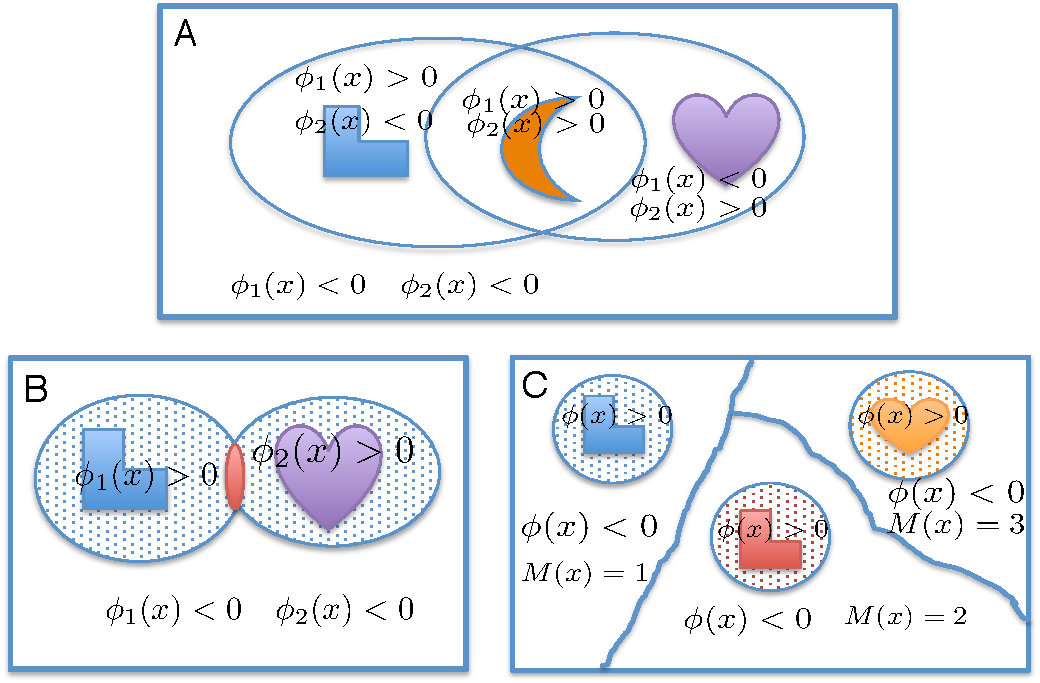
\includegraphics[width=1.0\textwidth]{images/imgseg_multiobjs}
\caption[The level set model of multi-objects segmentation]{A. Multi-phase level set model. B. Coupling $N$ level set model. C. Voronoi-Diagram base one level set model.}
\label{fig:imgseg-multiobjs}
\end{figure}
\section{My work}
The above image segmentation methods are from simple to complex, especially the last V-D based level set method, which is proposed by myself. I implement the method in C/C++. The test result shows its great potential on saving the running time significatly.
 % chapter1: image segmentation
\chapter{Component Tree}\label{chapter:cptree}
 % chapter2: component tree
\chapter{Tree assignment and tracking results} \label{chpt:treeassign}
Our cell tracking method needs to generate a bipartite matching \cite{mosig2009tracking, Xiao:2011} between consective component trees, which performs the role of both cell segmentation and cell association. In the most general form, generalizations of bipartite matching to trees have recently been shown to be $\mathcal{NP}$-hard\cite{canzar2011tree}.
In this thesis, we introduced two types of tree assignment problems. One is tree assignment between component trees, the other is tree assignment between neuron trees. Both models can be implemented by integer linear programming(ILP) and dynamic programming(DP). The two types of solution have different running time which depends on the complexity of tree structure. The tree assignment between trees with each node of few child nodes, such as component tree, is suitable to use DP, otherwise it is suitalbe to use ILP.

\section{Component tree assignment}
\subsection{Problem formulation}
Let $T_1$ and $T_2$ denote two rooted unordered trees, with vertices $U$ and $V$, respectively.  We refer to the set of all possible assignments between $T_1$ and $T_2$ as match $(T_1,T_2) =\Big\{M \subset U \times V | M = \{(u_1,v_1),\ldots,(u_k,v_k)\}\Big\}$. Given a weighting function $w:U\times V \to \mathbb{R}_{\le 0}$, we can assign a weight $W(M) := \sum_{u,v)\in M}w_{u,v}$ to an assisnment $M \in$ match$(T_1,T_2)$. Putting things together, this allows us to define the \emph{tree assignment problem}, which is to find the maximum weighted tree assignment $M$, given $T_1,T_2$ and $w$. The tree assignment problem is a generalization of maximum weighted bipartite matching problem.
\subsubsection{Three points condition}
We deal with tree assignments under \emph{three points condition} for component tree assignment base cosegmentation, which introduces a restriction on the topology of trees with three leaves. We adapt the recursions for the constrained tree edit distance to solve the restricted tree assignment problem.

The three-point condition involves the lowest common ancestor of two vertices $a,b$ in a tree, which we denote by lca$(a,b)$. Now, we defined the tree assignment matching $M \in$ match$(T_1,T_2)$ if for any tree assignments $(a_1,a_2),(b_1,b_2),(c_1,c_2) \in M$, we have
$$
lca(a_1,b_1) \preceq lca(a_1,c_1)  \Rightarrow lca(a_2,b_2) \preceq lca(a_2,c_2)
$$

Intuitively, the three-point condition ensures that for any tree pairs of vertices in an assignment, the topology of the two induced subtrees are in the same heirarchical order.  
\subsubsection{Component tree}
The component tree maintains the inclusion relationship between all possible connected component under all different threshold segmentation. Najman et al.\cite{Najman:04} introduced a quasi-linear algorithm to construct the component tree. And I introduced a pruning principle to simpify the component tree structure (see Chapter\ref{chpt:cptree}).

\subsubsection{Component tree weights}
The weight between two component nodes is defined as the ratio of overlapping size and union size. I introduced a quasi-linear dynamic algorithm to compute all the weights between two component trees (see Sec\ref{sec:cptree-weight}).
\subsection{Integer linear programming (ILP)}
Given two trees $T_1$ and $T_2$, to satisfy the \emph{three point condition}, we introduce the match $M \in$ match$(T_1,T_2)$ such that for any two distinct indices $1 \le i,j \le k$, neither $u_i$ is an ancestor/descendant of $u_j$ nor $v_i$ is an ancestor/descendant of $v_j$. 

For each vertex $u \in T_1, v \in T_2$, introduce binary variable $X_{uv}$, where $X_{uv} = 1$ iff $u$ is assigned to $v$, otherwise $X_{uv} = 0$. For any node $u, u' \in T_1$ and $v, v' \in T_2$, we can define the integer linear model with constraints,
\begin{equation}
\label{eqn:cptree-ilp-st}
\left\{
\begin{array}{l}
X(u,v) \in \{0,1\} \\
\forall u \preceq u', X(u,v) + X(u',v') \le 1 \\
\forall v \preceq v', X(u,v) + X(u',v') \le 1 
\end{array}
\right.
\end{equation}
and the objective function by maximum the sum of weight function,
\begin{equation}
 \max \sum_{u\in T_1, v \in T_2} w(u,v)X(u,v)
\end{equation}

For the constraints \ref{eqn:cptree-ilp-st}, the first constraint ensures the binary values for assignment variable, the second and third constraint ensure that only one node is matched in a leaf-node-to-root-node path in both trees (see Fig\ref{fig:treeassign-cptree}A and Fig\ref{fig:treeassign-cptree}B). 

Let $L(T)$ denotes all the leaf nodes of T; $root(T)$ denotes the root node of tree $T$; $path(u,v) = \{u_1 = u,u_2, \ldots, u_{n-1}, u_n = v\}$ denotes the path from node $u$ to node $v$; $P(T) = \{path(u, root(T))|u \in L(T)\}$ denotes all the leaf-node-to-root-node paths. The above constraints \ref{eqn:cptree-ilp-st} can be re-written as,
\begin{equation}
\left\{
\begin{array}{l}
X(u,v) \in \{0,1\} \\
\forall p \in P(T_1), \sum_{u\in p}\sum_{v \in T_2} X(u,v) \le 1 \\
\forall p \in P(T_2), \sum_{u\in T_1}\sum_{v \in p} X(u,v) \le 1 
\end{array}
\right.
\end{equation}

\subsection{Dynamic programming algorithms (DP)}


Jiang \cite{Jiang:95} provided a less constraint tree assignment algorithm.
For each $A \subseteq \{u_1,u_2,...,u_m\}$, $u_i \in T_1$ and each $B \subseteq \{v_1,v_2,...,v_n\}, v_j \in T_2$. \\
\begin{eqnarray} \label{eqn:lcdp-formular}
W(A,B) = \max \begin{cases}
\max_{a_i \in A, b_j \in B}(W(A-\{a_i\}, B-\{b_j\}) + w(a_i,b_j))\\
\max_{a_i \in A, B' \subseteq B}(W(A-\{a_i\}, B-B') + W(C(a_i), B')) \\
\max_{A' \subseteq A, b_j \in B}(W(A-A', B-\{b_j\}) + W(A', C(b_j))
\end{cases} 
\end{eqnarray}

Assume $r_1$ the root node of $T_1$ and $r_2$ the root of $T_2$, the solution of tree assignment will be $W(C(r_1), C(r_2))$.
Obviously the constrained tree assignment in section \ref{sect:tree-assignment} is covered as a special case by applying the first case of Eqn.\eqref{eqn:lcdp-formular}. 

\begin{figure}[htbp]
\centering
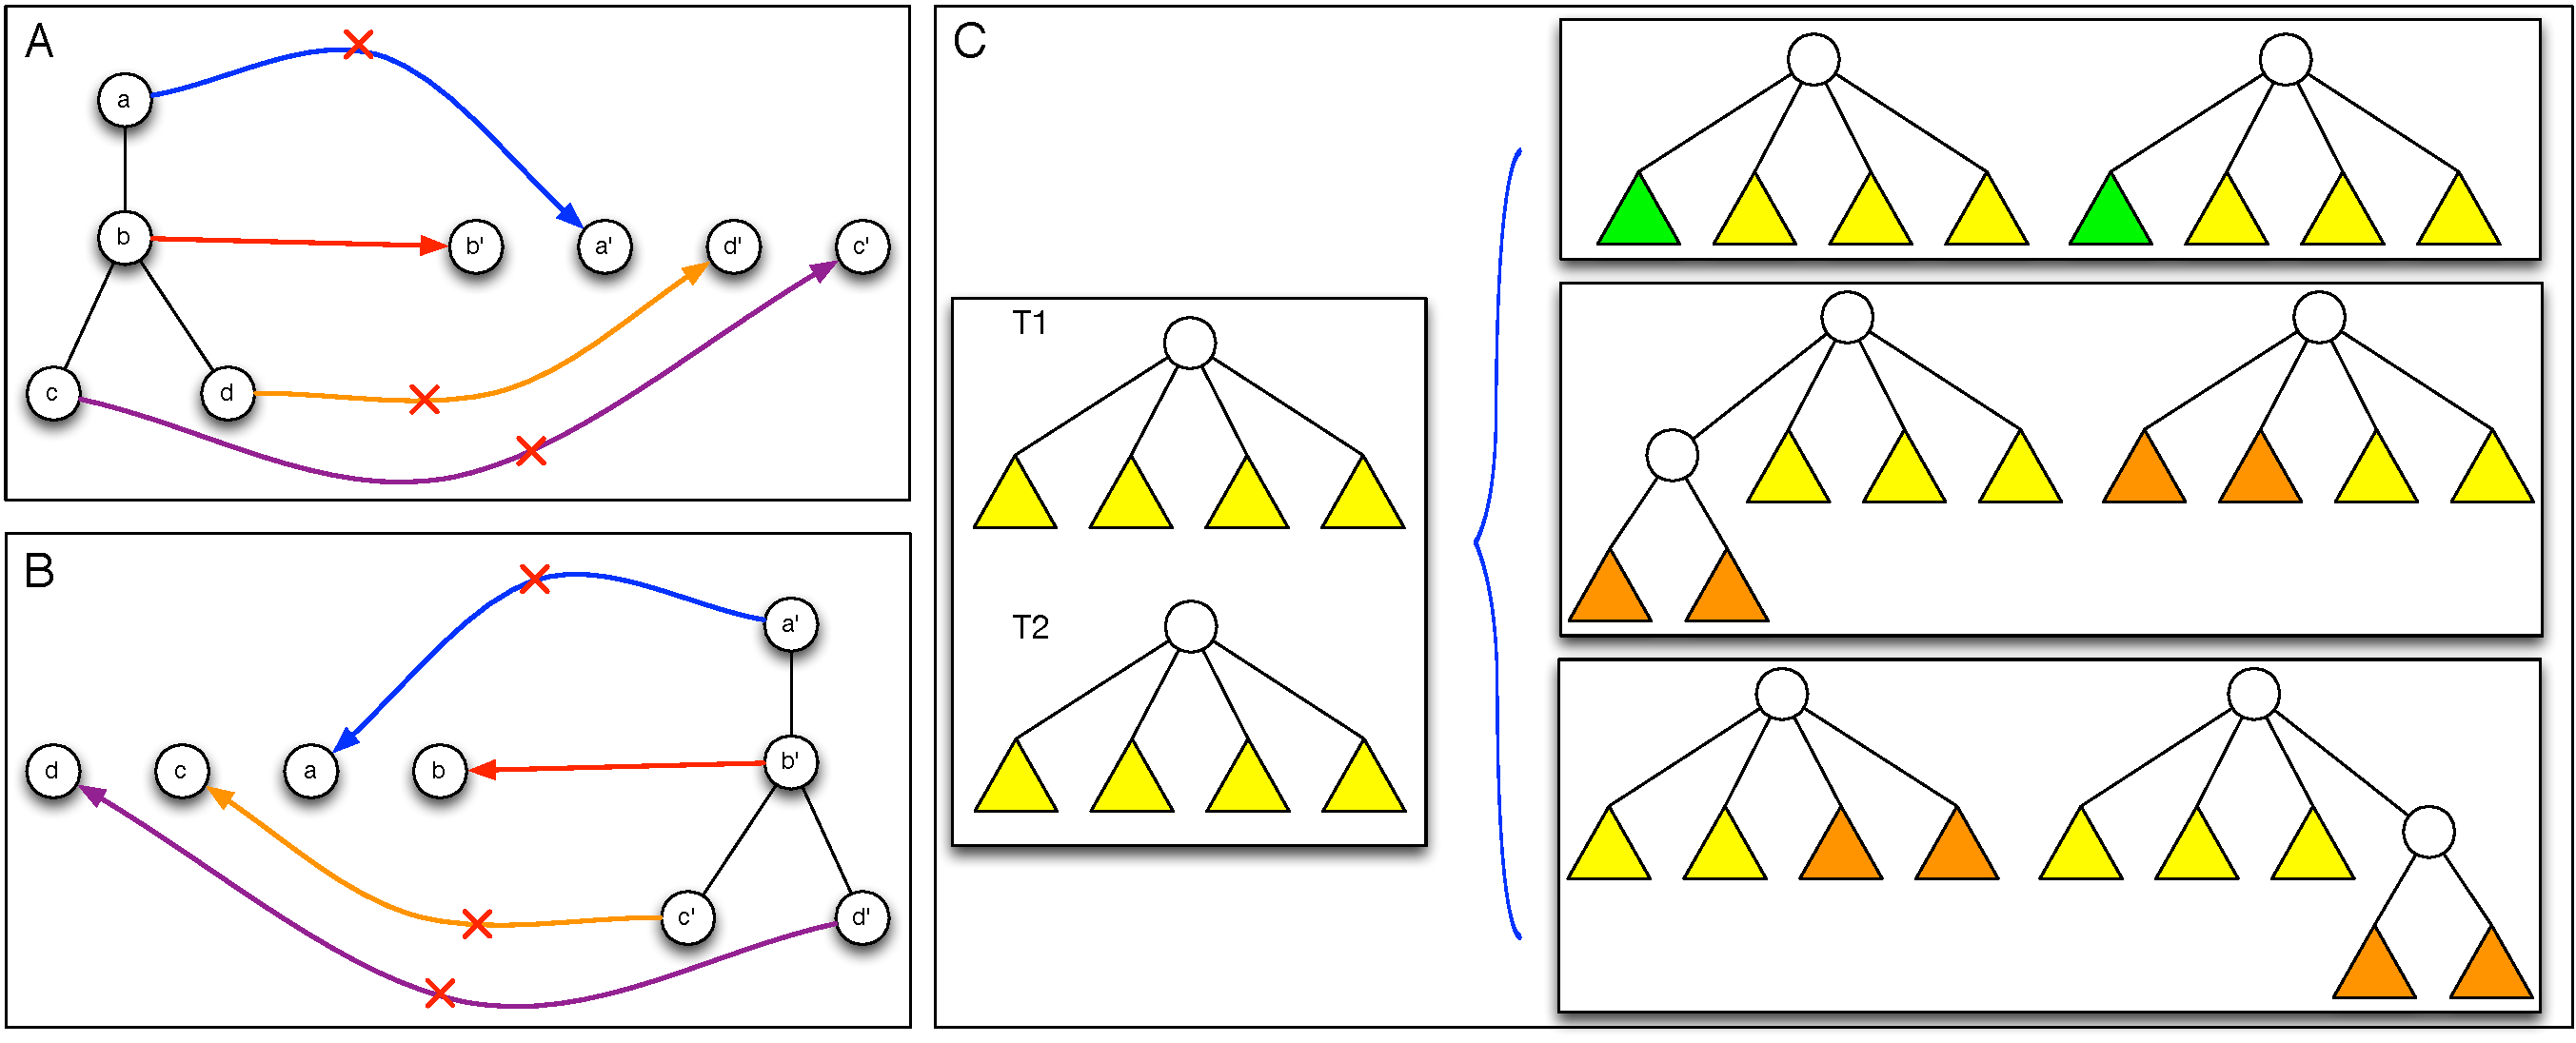
\includegraphics[width=1.0\textwidth]{images/treeassign_cptree}
\caption[ILP and DP models for component tree assignment]{ILP and DP models for component tree assignment. A. The second constraint in ILP model \ref{eqn:cptree-ilp-st} for component tree assignment; B. The third constraint in ILP model \ref{eqn:cptree-ilp-st} for component tree assignment; C. The DP model of component tree assignment.}
\label{fig:treeassign-cptree}
\end{figure}

\subsubsection{Running time}
With the less constrained recurrence, we will get much better result with higher mapping score. However, the time complexity turns out to depend exponentially on the maximum degree of the two trees
\begin{equation*} \label{eqn:lcdp-time}
O\left(\sum_{u_i \in T_1, v_j \in T_2}(2^{|C(u_i)|}\cdot 2^{|C(v_j)|})\right).
\end{equation*}
For binary trees, the running time will be
$O(|T_1|\cdot|T_2)$. \\
For component trees, the runing time will be 
$O\left(2^{|C(r_1)|}\cdot2^{|C(r_2)|}\right)$. \\
\subsubsection{Improvement}
Firstly we define the overlap between $A$ and $B$. We mean $A$ and $B$ have overlap that there exists some element in $A$ ovelaping with some element in $B$, otherwise no overlap.\\ 
When dealing with tree-assignments involving component trees, note that in practice many $A$ and $B$ have no overlap, or only few elements in $A$ overlap with few elements in $B$. The non-overlaping A and B can be neglected in the assignment. The overlaping A and B can be decomposed into disjoint subsets $A=A_0 \cup \ldots \cup A_n$ and $B = B_0 \cup \ldots \cup B_n$ such that $A_1 \cup B_1, \ldots, A_n \cup B_n$ are the connected components in graph $G(V, E)$ , that $V = A \cup B$ and $E = \{(a,b)|a \in A, b \in B, \beta(a) \cap \beta(b) \neq \emptyset\}$,  and $A_0$ and $B_0$ are the collection of isolated nodes of $A$ and $B$. As $A_0$ and $B_0$ can be neglected in the assignment, we have 
\begin{equation*} \label{eqn:ldcp-decomp}
W(A,B) = \sum_{k=1,\ldots,n}{W(A_k, B_k)}
\end{equation*}
In practice, $|A_k|$ and $|B_k|$ will be much smaller than $|A|$ and $|B|$, the runing time will be much smaller, which speed up the algorithm significantly on many instances.
\subsection{Difference between ILP and DP models}
Integer linear programming (ILP) and dynamic programming (DP) provide two different implementations for component tree assignment. DP model implements exactly the three point condition, three point condition fits the ILP model. However, ILP model doesn't always fit three point condition. Fig\ref{fig:treeassign-threepoint}A illustrates the match result in ILP which doesn't fit the three point condition. Fig\ref{fig:treeassign-threepoint2} shows the match difference between ILP and DP, where the segmentation results if ILP contain that of DP.

\begin{figure}[htbp]
\centering
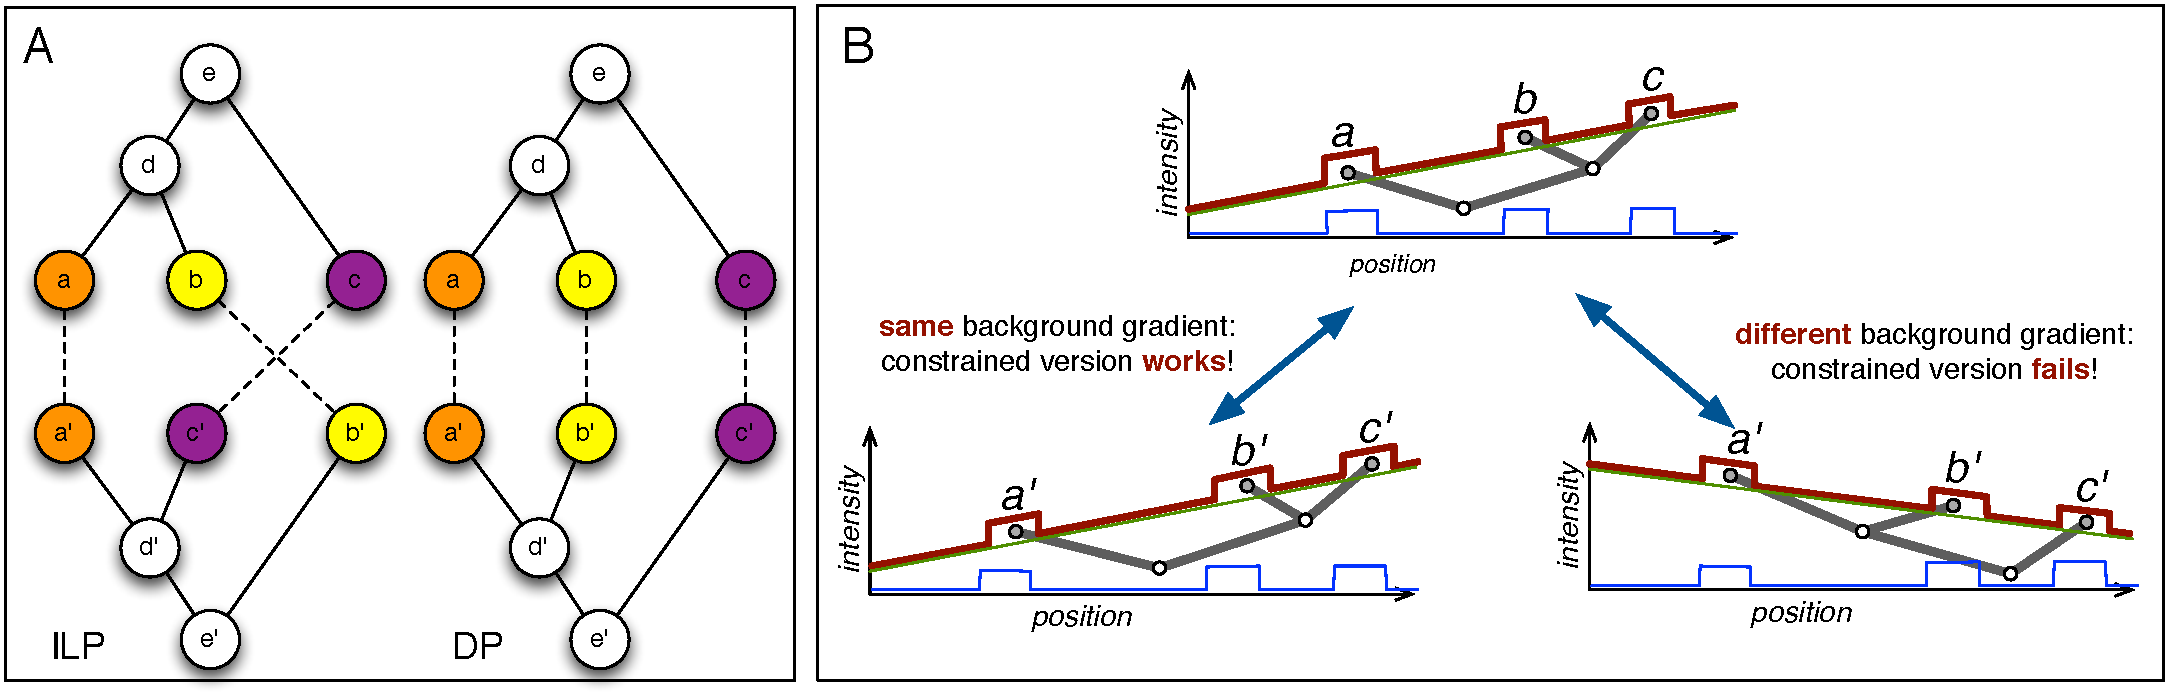
\includegraphics[width=1.0\textwidth]{images/treeassign_threepoint}
\caption[Three point condition]{A. The difference between ILP and DP models, where DP fits exactly three point model, while ILP extends three point condition; B. The explaination of three point condition which is especially efficient when background gradient.}
\label{fig:treeassign-threepoint}
\end{figure}

\begin{figure}[htbp]
\centering
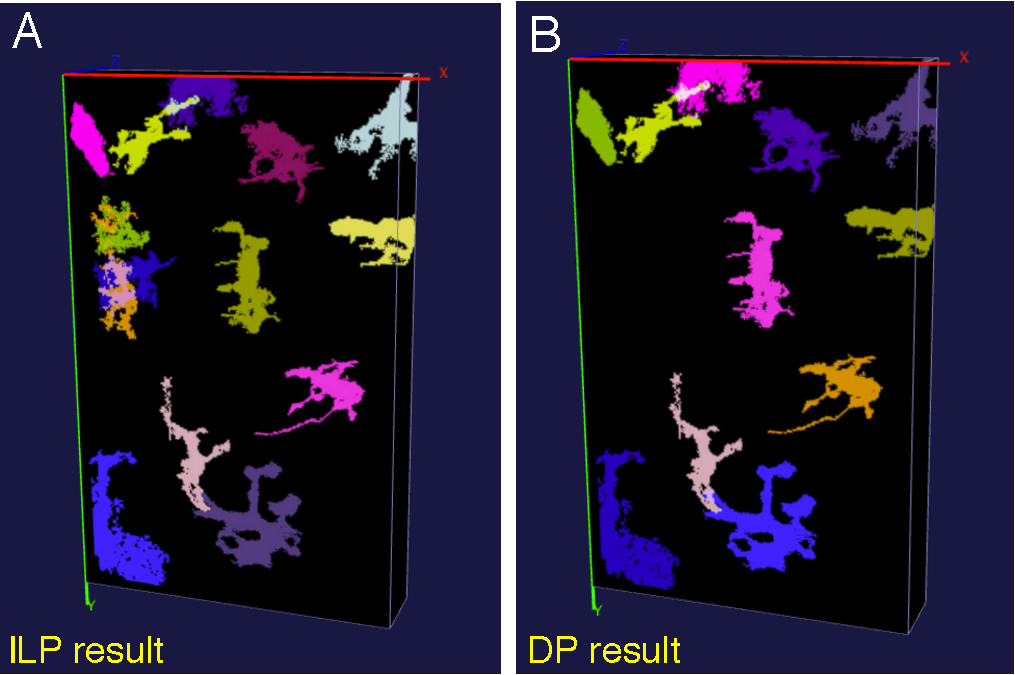
\includegraphics[width=1.0\textwidth]{images/treeassign_threepoint2}
\caption[ILP and DP result difference for microglia cell segmentation]{ILP and DP result difference for microglia cell segmentation, the red circles indicate the additional match result of ILP model.}
\label{fig:treeassign-threepoint2}
\end{figure}

\subsection{A model for cell spliting and merging}
The proposed algorithms can only track the movement of cell without cell splitting and cell merging, as the algorithms descirbed above assign the node in one tree to exactly only one node in the other tree. Both ILP model and DP model will loose the track of cells if cell splitting or cell merging exist. (Usually only cell splitting exists in practice.) We improve the linear tree assignment model that each node in one tree can be assigned to many nodes in the other tree. However, the constraint that only one node is assigned in a leaf-to-root-node path is kept. 

Given two trees $T_1$ and $T_2$, for each vertex $u \in T_1$, $v \in T_2$, we introduce additional two binary variables $Y_u$ and $Z_v$ besides $X_{uv}$. $X_{uv} = 1$ if node $u$ is assigned to node $v$, otherwise $X_{uv} = 0$. If node $u$ is assigned to any node in $T_2$, $Y_u = 1$; and $Y_u = 0$ if node $u$ is not assigned. The same rule works for $Z_v$. The relationship between $Y_u$,$Z_v$ and $X_{uv}$ is given by,
\begin{equation}
	Y_u = 
	\left\{
	\begin{array}{cc}
		0 & \text{if \quad $\sum\limits_{v \in T_2}X_{uv} = 0$} \\
		1 & \text{if \quad $\sum\limits_{v \in T_2}X_{uv} \ge 1$}
	\end{array}
	\right.
	\quad \text{for $u \in T_1$}
\end{equation}
\begin{equation}
	Z_v = 
	\left\{
	\begin{array}{cc}
		0 & \text{if \quad $\sum\limits_{u \in T_1}X_{uv} = 0$} \\
		1 & \text{if \quad $\sum\limits_{u \in T_1}X_{uv} \ge 1$}
	\end{array}
	\right.
	\quad \text{for $v \in T_2$}
\end{equation}
By considering the condition that only one node is assigned for a leaf-node-to-root-node path, the integer linear model is given by
\begin{equation}
\left\{
\begin{array}{l}
\sum\limits_{u \in P1 \in P(T_1)}Y_u \le  1 \\
\sum\limits_{v \in P2 \in P(T_2)}Z_v \le  1 
\end{array}
\right.
\end{equation}
with the same objective function
\begin{equation}
max\sum\limits_{i \in T_1}\sum\limits_{j \in T_2}w_{ij}X_{ij}
\end{equation}

The constraints for $Y_i$ and $Z_j$ is not clear, which seems like a non-linear interger programming. However there are two kinds of methods to define $Y_i$ and $Z_j$ and turn the problem into linear integer programming.

\textbf{Method 1:}
\begin{eqnarray}
\frac{\sum_{v \in T_2}X_{uv}}{|T_2|} \le Y_u \le \sum_{v \in T_2}X_{uv} & \text{for $u \in T_1$} \\
\frac{\sum_{u \in T_1}X_{uv}}{|T_1|} \le Z_v \le \sum_{u \in T_1}X_{uv} & \text{for $v \in T_2$}
\end{eqnarray}
Obviously when $\sum\limits_{u \in T_1}X_{uv}$ equals to zero, $Y_u$ will less than zero, due to the \{0,1\} constraint, $Y_u$ will be zero. When $\sum\limits_{u \in T_1}X_{uv}$ larger than zero,beacuse of $\sum\limits_{u \in T_1}X_{uv}$, $Y_v$ always no greater than $|T_1|$, $Y_u$ will larger then a value, which is larger then zero and no greater than 1. So $Y_u$ will of course be one. This contrains fit the definition of $Y_u$ very well. The contraint also fit to $Z_v$ very well.

\textbf{Method 2:}
\begin{eqnarray}
Y_u \ge X_{uv} &\text{for each $v \in T_2$, for $u \in T_1$}\\
Z_v \ge X_{uv} & \text{for each $u \in T_1$, for $v \in T_2$}\\
\label{con:multi-align1}
Y_u \le \sum\limits_{u \in T_1}X_{uv}  & \text{for $u \in T_1$}\\
\label{con:multi-align2}
Z_v \le \sum\limits_{v \in T_2}X_{uv}  & \text{for $v \in T_2$}
\end{eqnarray}
Once node $u \in T_1$ and node $v \in T_2$ is matched, $X_{uv}$ will be one, and $Y_u$ and $Z_v$ will be no less than $X_{uv}$, so $Y_u$ and $Z_v$ both will be 1. The constraints \ref{con:multi-align1} and \ref{con:multi-align2} is used for nonmatching instances. If node $u \in T_1$ or node $v \in T_2$ is not matched at all, $Y_u$ or $Z_v$ will be 0 either. So now the method 2 fit the definition of $Y_u$ and $Z_v$ perfectly.

\section{Neuron tree assignment}
\subsection{Two points condition}
\subsection{Optimization formula}
\subsection{Integer linear programming}
\subsection{Dynamic programming algorithms}
\section{Cell Tracking results}
 % chapter3: Tree assignment methods
\chapter{Cell tracking methods}
based on \cite{Xiao:2011}
 % chapter4: cell tracking methods
\part{Neuron Tracing}
\chapter{Fast marching method} \label{chpt:fm}
Fast marching(FM) method \cite{sethian1999level} plays a very important part in both automatic neuron tracing (APP2 method) and human-guided neuron tracing. It is essentially a region-growing scheme and can be used for GSDT and initial neuron reconstruction in APP2 and finding shortest path between rays in human-guided neuron tracing.
\section{Introduction}
\subsection{Algorithm flow}
In FM, we model an image as a graph, where each graph vertex corresponds to an image pixel (voxel). There is an edge between each pair of immediately neighboring pixel-vertices. FM grows the image graph from a set of predefined seed vertices to all remaining image pixel-vertices in a distance-increasing order.  All image pixels are divided into three groups, labeled as \emph{ALIVE}, \emph{TRIAL} and \emph{FAR}. 

FM has two main steps: initialization and recursion. First, all the seed vertices are initialized to be \emph{ALIVE}; the neighbors of seeds are initialized as \emph{TRIAL}; and the rest are set as \emph{FAR}. Then, from the set of \emph{TRIAL} vertices, we will extract one vertex x, which has the minimum distance value to the \emph{ALIVE} set. The extracted vertex x is then converted from \emph{TRIAL} to \emph{ALIVE}.  For any non-\emph{ALIVE} neighbor y of x, we set it to \emph{TRIAL} if it is \emph{FAR}. The distance function of y is updated as (also see below for concrete definitions)
\begin{equation}
d(y)=\min⁡{d(y),d(x)+e(x,y)}
\end{equation}

where $e(x,y)$ is the distance between vertex $x$ and vertex $y$ (see below for definition of $e(x,y)$). FM recursively extracts the vertex that has the minimum-distance from the \emph{TRIAL} set until it becomes empty.
An important implementation trick of FM is to maintain \emph{TRIAL} vertices in a Fibonacci heap so that the required minima can be obtained efficiently. See Alg.\ref{alg:fast-marching} for the algorithm flow of FM.

\begin{algorithm}[H]
\label{alg:fast-marching}
\SetKwInOut{Input}{Input}\SetKwInOut{Output}{Output}
\SetAlgoLined
\Input{seed points $x_0,x_1,\ldots,x_n$}
\Output{Return distance map $d(x)$}
Initialize distance map $d(x) = \infty$ for all point and mark as \emph{FAR} \;
Initialize $d(x_0),d(x_1),\ldots,d(x_n)$ to $0$ and mark it as \emph{ALIVE} \;
Initialize queue of \emph{TRIAL} points $Q = \O$ \;
Mark \emph{FAR} neighbors of \emph{ALIVE} points as \emph{TRIAL} (add to $Q$) and update $d$ \;
\While{Q is not empty}{
Remove minimum point $x$ from $Q$, mark $x$ as \emph{ALIVE}\;
Mark \emph{FAR} neighbors of $x$ as \emph{TRIAL} and insert into $Q$\; 
Update $d$ for the neighbors of $x$\;
}
\caption{Fast marching algorithm}
\end{algorithm}

\subsection{Differnce from dijkstra's algorithm}
In general, fast marching method is the same to Dijkstra's algorithm except that FM applys dynamic weight function. In fast marhcing method, the weight for each edge can be calculate when the edge is under marching.
\section{Applications}
Fast marching method can be applied to many bio-image processing according to the number of seed points, the definition of edge length $e(v_0,v_1)$ and the output information. The number of seed points for fast marching can be single or multiple. The edge length $e(v_0,v_1)$ can be defined as,
$$
e(v_0,v_1) = \left\{ 
    \begin{array}{lr}
    ||v_0 - v_1|| & \mbox{Euclidean distance (1)} \\
    \\
    ||v_0 - v_1|| \cdot (g_I(v_0) + g_I(v_1))/2 & \mbox{Geodesic distance (2)} \\
    \\
    ||v_0 - v_1|| \cdot (I(v_0) + I(v_1))/2 & \mbox{Image intensity (3)} \\
    \\
    f(v_0,v_1) & \mbox{other distance (4)}
    \end{array}
    \right.
$$
In the right column, $I(v)$ is image intensity at location $v$, $g_I(v)$ is expontial to image intensity $I(v)$, $f(v_0,v_1)$ is predefined distance map. The output information after fast marching may be distance map or parental map.  The related applications is classfied in tab.\ref{tab:fm-app}.\\

\begin{table}
\begin{center}
\begin{tabular}{ | c | c | c | c |}
    \hline
    \textbf{Application} & \textbf{Num of seeds} & \textbf{Edge length} & \textbf{Output} \\ \hline
    neuron reconstruction & single & geodesic distance & parental map \\ \hline
    GSDT & multiple & image intensity & distance map  \\ \hline
    3D curve drawing & multiple & geodesic distance & both \\ \hline
    Voronoi diagram & multiple & euclidean distance & parental map  \\ \hline
    seeded watershed & multiple & predefined & parental map \\ \hline
  \end{tabular}
\end{center}
\caption{This table shows some data}
\label{tab:fm-app}
\end{table}

\subsection{3D curve drawing}
\label{sect:fm-3dcurve}
Draw 3D curve is a post-processing step to correct the tracing errors during automatic neuron tracing \cite{peng2011automatic, Xiao:2011}. VAA3D \cite{peng2010v3d} provides a solution to select a 3D marker by one or two mouse click(s). However, it is not realistic to choose 3D markers one by one to draw a 3D curve. The convinient operation is to draw a 3D curve on 2D projection plane directly. Accuately, a drawing curve on 2D projection plane is lots of parallel sampling rays (see Figure \ref{fig:fm-dynamic-drawing}A), which are perpendicular to the projection plane. There exist lots of potiential 3D curves corresponding to the drawing curve. To get the exact 3D curve that we want, one possible solution is to draw the 3D curve twice from different views and then we find the intersection points. However, this is not a perfect solution as it needs too many drawing operations.

To find the 3D curve (see Figure \ref{fig:fm-dynamic-drawing}B) that is exactly what we want,  VAA3D provides some solutions for the problem. The main idea in VAA3D is to estimate the 3D position for each sampling ray by using meanshift \cite{comaniciu2002mean} algorithm. However, for complex background noise, meanshift may fail to find the correct 3D position(see Figure \ref{fig:fm-meanshift-drawing}B), as meanshift will attract to local maximum center when strong background noise exists. 

Here, we provide a method to solve curving drawing problem, which contains two novel ideas. First idea is to find the shortest path between two rays, which is solved under fast marching framework. Second idea is to find the shortest path that accross all sampling rays, which is assumed to be the expected 3d drawing curve.

\subsubsection{Shortest path between two rays}
This problem can be perfectly sovled by fastmarching method. Assume we draw the curve from subject ray to target ray. Firstly, all the vertices on the subject ray will be used as seed points. Then marching from the seed points until all vertices on the target ray are marched. From the resulting distance tree, we can easily get the shortest path by reverse from each vertex on the target ray until the first vertex on the source ray is visited. In practice, there is no need to march all vertices on the target ray; normally when 50\% vertices are marched, the marching process can stop.

The length between consective vertices (or points) $v_0$ and $v_1$ is defined as, 
$$
e(v_0,v_1) = ||v_0 - v_1||\cdot \left( \frac{g_I(v_0) + g_I(v_1)}{2} \right)
$$
which is the geodestic distance widely used in neuron tracing \cite{peng2010automatic, peng2011automatic}. $g_I(v_i)$ on the right item is defined as ,
$$
g_I(v_i) = exp(\lambda_I(1-I(v_i)/I_{max})^2)
$$
where $I(v_i)$ is the intensity of vertex $v_i$ and $I_{max}$ is the maximum intensity of the entire image $I$. So the edge length between bright points will be very small, which ensure the shortest path go accross the continuous bright points as much as possible.

\textbf{Extension:} The method for finding the shortest path between two rays is easily extended to finding shortest path between two groups of any points. The rays above is not restricted to parallel rays.

\subsubsection{Shortest path between multiple rays}
Like the shortest path between two rays, there exist a shortest path that connect multiple rays. One way to connect multiple rays is to simply connect consecutive rays by the shortest path between them. For each non-start/non-end ray, there are two shortest paths connect to it. The problem arises that the two shortest paths are mostly probably not connected, that we still need to connect the two shortest paths which increase the total cost. To solve the problem of disconnected shortest paths, we can use the end point of last shortest path as the start point of the next shortest path instead of starting from a whole ray.

The above suggestions may find a good path but not the global shortest path. To find the global shortest path, we proposed the following steps.
\begin{itemize}
\item[a.] find all shortest path from first ray to each vertex on the second ray
\item[b.] keep the distance value on the second ray and find the shortest path from the second ray to each vertex on the third ray
\item[c.] iterate the above step until the last ray is reached
\end{itemize}

Usually we don't need to assure all vertices on a ray are reached, as some vertices are very time consuming to reach. In practice, we set 50\% vertices reached  to start the next iteration.
\subsubsection{Further optimization for multiple rays}
The abolve global shortest path is not always good when the sampling ray deviated to background (see Figure \ref{fig:fm-dynamic-compare}C). Actually, the sampling ray should be used as a reference to indicate that the 3D curve should near to the ray. For consective rays, we can set a bounding box. So we can change the model as the 3D curve is the shortest path from the first ray to the last ray by accrossing the boudingboxes between consective rays (see Figure \ref{fig:fm-dynamic-compare}B). We can see the different drawing results with same sampling rays, Fig.\ref{fig:fm-dynamic-compare}C for original model and Fig.\ref{fig:fm-dynamic-compare}D for improved model. The original model may produce lots of spurs near sampling rays while the impoved model produces much smoother result.
%\includegraphics{2_dynamic.pdf}

\begin{figure}[htb]
\begin{center}
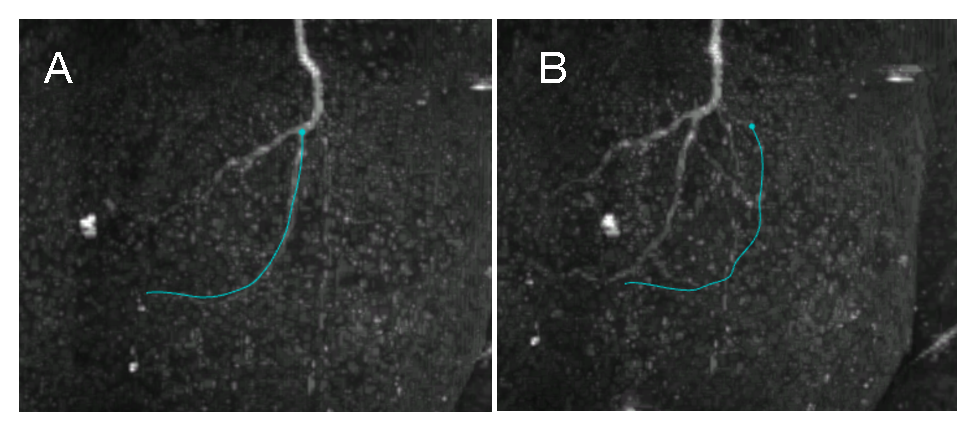
\includegraphics[width=5in]{images/fm_meanshift_drawing}
\caption{(A) meanshift based curve drawing. (B) error occured on noisy background}
\label{fig:fm-meanshift-drawing} % \lable should be after \caption
\end{center}
\end{figure}

\begin{figure}[htb]
\begin{center}
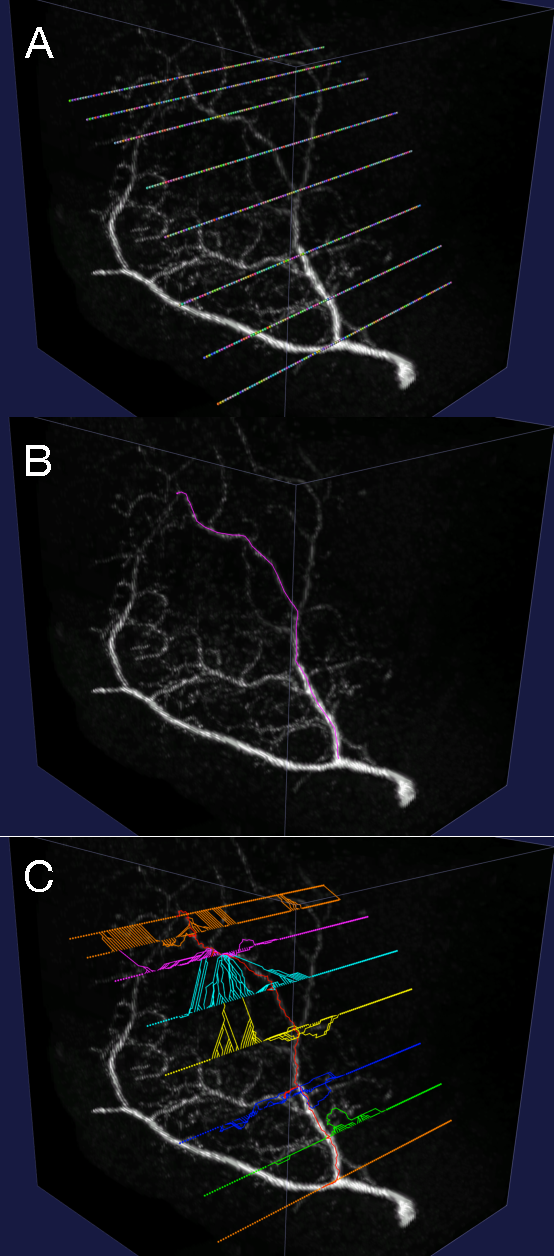
\includegraphics[width=4in]{images/fm_dynamic_drawing}
\caption{(A) sampling rays. (B) expected 3D curve. (C) the process of global optimized model}
\label{fig:fm-dynamic-drawing}
\end{center}
\end{figure}

\begin{figure}[htb]
\begin{center}
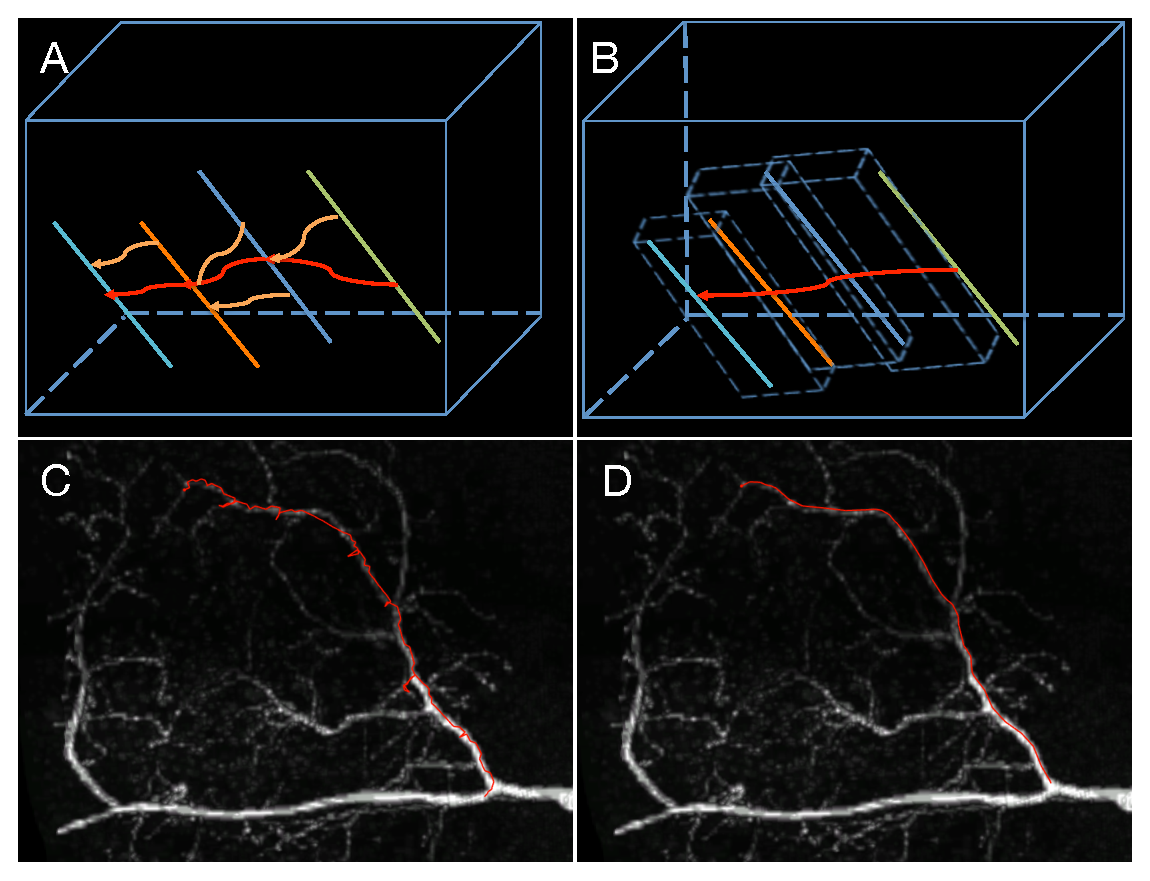
\includegraphics[width=5in]{images/fm_dynamic_compare}
\caption{(A) global optimized model. (B) improved bounding-box model (C) the result or original model. (D) the result of improved model}
\label{fig:fm-dynamic-compare}
\end{center}
\end{figure}
\subsection{Gray-weighted distance transform}
Normally, the distance transform is perform on binary image. The distance for each foreground point is the minimum euclidean distance to background. To perform distance transform on grayscale image, we can define the distance for each foreground point as the length of its shortest path to background. The length of a path is the sum of gray value of the point on the path. This idea is called gray-weighted distance transform (GWDT) \cite{rutovitz1968data}. To implement this idea, we need to use fast marching method and dynamic programming, for the detail of GWDT, see section \ref{sec:gwdt}.

\subsection{Generalized Voronoi diagram for shapes} \label{subsec:gvd}
In image processing, a Voronoi diagram \cite{aurenhammer1991Voronoi} is a special kind of decomposition of an image, determined by distances to a group of specified objects. These objects can be many seed points (Figure \ref{fig:fm-Voronoi}A) normally or many cell bodies (Figure \ref{fig:fm-Voronoi}B). The Voronoi Diagram for cell bodies is also called Generalized Voronoi Diagram (GVD) \cite{nath2007accurate}. The decomposted image areas are Voronoi areas. Each Voronoi area is a group of points whose nearest object are the same. Voronoi Diagram can be found in a large number of fields in science and technology, even in art.\\
There are lots of algorithms proposed to solve the Normal Voronoi Diagram. Lloyd \cite{lloyd1977triangulations} firstly consider the problem as a k-means clustering problem. A more efficent algorithm for generating a Voronoi Diagram in a plane is proposed by Fortune \cite{fortune1987sweepline} in $O(nlog(n))$ time. The method need to scan the image from left to right with a sweep line. For higher dimension image, Bowyer Watson \cite{rebay1993efficient} proposed a method to solve the complementary problem Delaunay triangulation in any number of dimensions. However, these algorithms only solve the Normal Voronoi Diagram problem. For the Generalized Voronoi Diagram problem, there isn't efficient methods \cite{hoff1999fast, takahashi1989motion, nath2007accurate}. Actually either normal Voronoi diagram or generalized Voronoi diagram problems can be considered as a shortest path problem by growing seed points or cell bodies to nearest area. It is a fast marching problem. The only thing we need to do is labeling each object with unique lable. Each pixel will be labeled the same to its nearest object.

\begin{figure}[htb]
\begin{center}
\includegraphics[width=4in]{images/fm_Voronoi}
\caption[Normal Voronoi diagram and generalized Voronoi diagram]{(A) sampling rays. (B) expected 3D curve. (C) the process of global optimized model}
\label{fig:fm-Voronoi}
\end{center}
\end{figure}

\chapter{Hierarchical pruning based automatic neuron tracing methods} \label{chpt:auto-nt}
In this chapter we focus on neuron tracing for 3D light-microscopic images (often confocal or multi-photon laser scanning microscopic images). Taking a 3D gray-scale image as the input, a neuron trac-ing method produces the digital representation of the morphology of the neuron(s) in this image. Tracing multiple neurons that poten-tially overlap in an image has been found to be fundamentally ill-posed and might be ultimately tackled using biological tissue label-ing methods, such as dBrainbow \cite{hampel2011drosophila}. In the latter case, the problem reduces to tracing of a group of single-channel images, each of which contains a single neuron. Therefore, here we discuss only how to reconstruct a single neuron’s morphology from an image. 
\section{Overview}
\subsection{Local/Global neuron tracing methods}
\subsection{APP1 method}
\section{APP2 method}
\subsection{Overview of APP2}
In many previous studies, the 3D reconstructed morphology of a neuron is described using a tree graph $G$.  $G$ has a root node that corresponds to the seed location for reconstruction, which in many cases also corresponds to the soma of a neuron. $G$ may also contain many leaf nodes, branching nodes and other inter-nodes.

An important idea in the recent all-path-pruning (APP) method \cite{peng2011automatic} is to first generate an over-reconstruction from the image to capture all possible signal/pixels of a neuron, and then uses an optimal pruning procedure to remove the majority of spurs in this over-reconstruction to produce a final succinct representa-tion of the neuron, with a maximum coverage of all neuron signal. The pruning process starts from leaf nodes of the over-reconstruction. A "coverage" test is iteratively conducted to check whether or not any of them have been "covered" (i.e. has signifi-cant signal overlap) by other nodes. The nodes that are covered by others will be removed; otherwise they will be kept. A similar process is also applied to all internodes. The entire procedure is repeated until a most succinct representation that maximizes the signal coverage has been produced. While the termini-first-search approach in APP is effective, it needs multiple iterations, which could still be time-consuming even the algorithm itself has linear-time complexity to the number of reconstruction nodes. In addi-tion, APP does not consider how to best preprocess an input image to optimize the tracing result. 

APP2 follows the basic framework of APP. However, it enhanc-es the key components of the original method. In short, APP2 con-sists of three steps in Fig.\ref{fig:autont-fig1}b, c, and d: (1) gray-weighted distance transform (Section \ref{sec:gwdt}); (2) construction of an initial, over-reconstruction of the traced neuron (Section \ref{sec:init-nt}); and (3) pruning of the over-reconstruction in hierarchical order (Section \ref{sec:nt-hp}). The detail of APP2 is described as follows.

\begin{figure}[htbp]
\centering
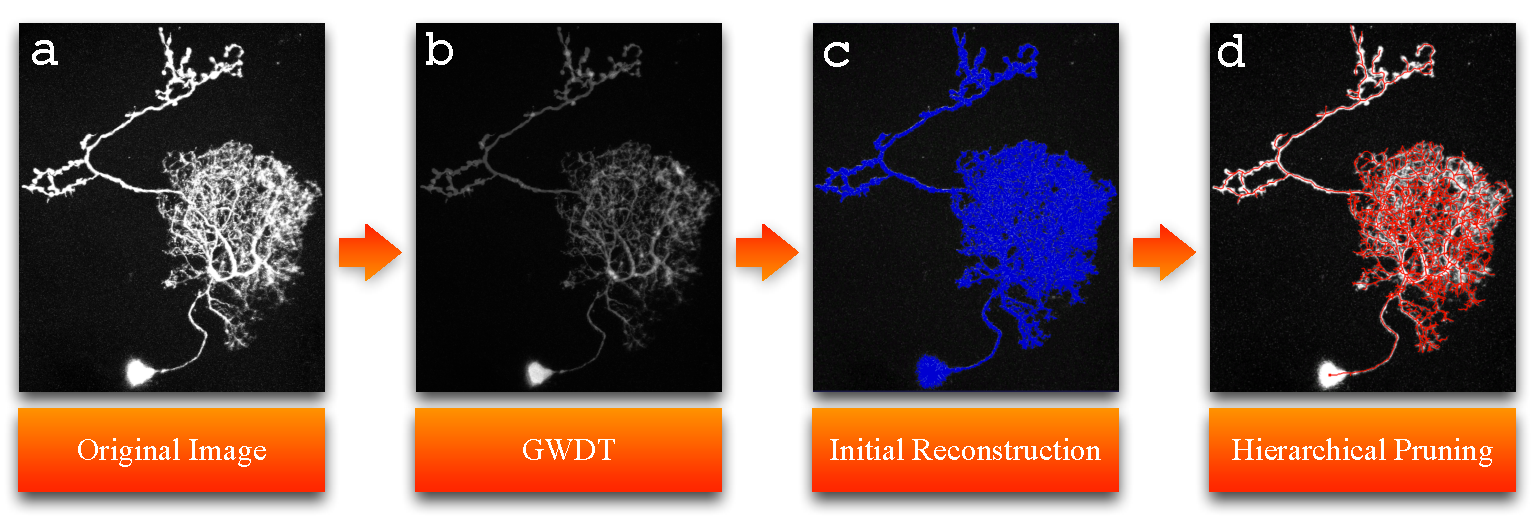
\includegraphics[width=1.0\textwidth]{images/autont_fig1}
\caption[Schematic illustration of APP2 neuron tracing method]{Schematic illustration of APP2 neuron tracing method. GWDT: gray-weighted distance transform. In c and d, the reconstructions are color-rendered and overlaid on top of the image data for better visualization. Raw image: Courtesy of Chiang lab.}
\label{fig:autont-fig1}
\end{figure}
\subsection{GWDT: Gray-Weighted Distance transfrom} \label{sec:gwdt}
To enhance the quality of an initial neuron reconstruction, in APP2 we apply the distance transform (DT) to the input image. In case of an image region that have relatively "flat" intensity, DT is able to create a gradient of image intensity: close to the center of this region the image intensity is large, and close to the boundary the intensity is small. We call this ICDB principle, which stands for "\emph{i}ncrease the intensity in the \emph{c}enter and \emph{d}ecrease the intensity near \emph{b}oundary". It would help to build a high quality initial reconstruction by forcing the shortest path to go through the skeleton of the neuron.

However, the conventional distance transform is only applicable to a binary image that is produced by thresholding a gray-scale image. An unsuitable threshold may under or over segment the image. Here we propose a gray-weighted distance transform method for gray-scale image (GWSDT) directly. In the conventional distance transform, the distance value for each image pixel is defined as the minimal Euclidean distance to background pixels. In GWSDT, the distance value for each pixel is defined as the sum of image pixels’ intensity along the shortest path to background. This is intrinsically similar to the gray weighted distance transform that has been previously defined by Rutovitz (1968)\cite{rutovitz1968data} and its variants. Most of the previous work and implementations (such as the recently released Matlab toolbox function) were limited to 2D cases, while our method and implementation are general for N-dimensional data ($N = 2,3,\ldots$). In the following we describe our fast implementation within FM framework.   

The distance value defined in GWSDT fits the ICDB principle. To use GWSDT, we often use a very low threshold value (e.g. the average intensity of an entire image). Any image pixels that have intensity value no greater than this threshold are called "background pixels". We first set all image background pixels as "seeds", then compute the distances from these seed pixels to other pixels. This process is similar to region growing, and thus is formulated within the FM framework in Chapter \ref{chpt:fm}. Here, the edge distance between consecutive image pixel vertices is defined as,
\begin{equation}
e(x,y)=|(|x-y|)|.I(y)
\end{equation}
Where $x$ is source vertex, $y$ is target vertex, $I(y)$ is the intensity of image pixel $y$. Let $d(x)$ denote the distance value of $x$. In the initialize step, we set
\begin{equation}
d(x)= \left\{
\begin{array}{rl}
I(x)  & x \in {background} \\
\infty &    x \notin {background } 
\end{array}
\right.
\end{equation}
We will set all background pixels as seeds. The neighbor pixels of all seeds will be set as the initial \emph{TRIAL} vertices and are pushed into the priority queue. In the growing step we will apply the formula,
\begin{equation}
d(x)=\min⁡{d(y)+ I(x)},y \in \{\mbox{neighbors of }x\}
\end{equation}
to refresh the distance value from background to skeleton center.

\textbf{Automated Soma detection}: We find that GWSDT method provides a way to detect the soma position of a neuron. Normally the soma has the maximum distance-transformed value (e.g. see results in \ref{}).

\subsection{Initial neuron reconstruction}\label{sec:init-nt}
In APP, the initial neuron reconstruction is essentially produced via finding the single-source (often from the soma) shortest path to all remaining foreground image pixels. APP uses Dijkstra’s algorithm, which needs to first build a graph of all foreground pixels and then find the shortest path from each pixel to the seed. For very large 3D image stacks, this approach may need a large amount of computer memory to hold the graph. In APP2, we present a new method to use FM to construct the initial reconstruction (Fig. \ref{fig:autont-fig2}), without the need to create such a large graph. 

In our implementation, we add a parental map par on the FM as described in Chapter \ref{chpt:fm} to generate the shortest path tree from a single source s.  Initially, the parent of each image pixel $x$ is set to be itself, i.e. $par(x)=x$. Then, for each neighbor pixel $y$ of $s$, we set them to have label "\emph{TRIAL}", and at the same time $par(y)=s$. In the recursive step, for the minimum pixel $x$ and each of its neighbor $y$, we set
\begin{equation}
par(y) = \left\{
\begin{array}{cl}
x & \mbox{if }y\mbox{ is }FAR \\
x & \mbox{if }d(x)+ e(x,y)< d(y)
\end{array}
\right.
\end{equation}

The edge distance e(x,y) is defined as the geodesic distance,
\begin{equation}
e(x,y)=\parallel x-y\parallel\cdot((g_I (x)+ g_I (y))/2)
\end{equation}
where the first item is Euclidean distance of the two pixels, and $g_I (.)$ in the second item is defined in the same form of APP \cite{peng2011automatic}, where $λ_I$ is a coefficient (set as 10 throughout our tests). 
\begin{equation}
g_I (x)=exp⁡(λ_I (1-I(x)/I_{max} )^2 )
\end{equation}
When FM has finished, we can build the initial reconstruction from the parental map.

In addition to the small working space needed, another useful property of FM for generating the initial reconstruction is that it can be stopped easily as needed. We consider two methods in APP2. First, the recursive step will stop when any background pixel becomes \emph{ALIVE}. This method prevents the marching process growing to any irrelevant area. Second, a user can optionally choose to specify some locations in advance (e.g. some special termini of a neuron) as additional priors; when all of these special locations have been labeled as \emph{ALIVE}, FM stops. The second method forces FM to reach these specified locations. Both methods are used in practice to generate complete initial reconstructions that cover signals as much as possible and thus make it easier to trace broken pieces or gaps in images. 

\begin{figure}[htbp]
\centering
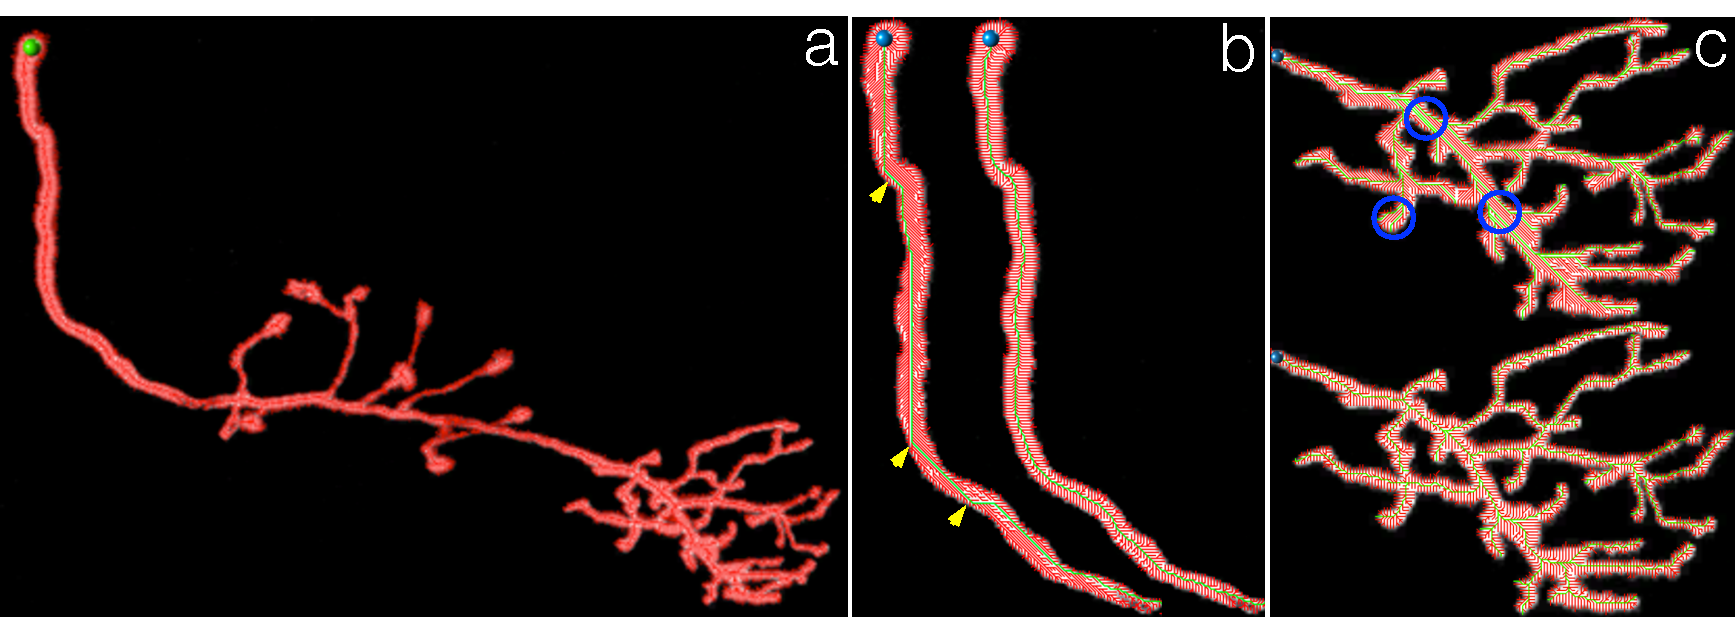
\includegraphics[width=1.0\textwidth]{images/autont_fig2}
\caption[Initial reconstruction based on GWDT and comparison results with or without GWDT]{Initial reconstruction based on GWDT (image: DIADEM OP1) and comparison results with or without GWDT. (a) The main GWDT-based skeleton (the major mid-curves) of the tracing implies a good tracing.  Sphere: the seed location. (b) left: out-of-center problem without GWDT preprocessing; right:  main structure goes to the neuron center with GWDT preprocessing . (c) top: parallel-path problem without GWDT preprocessing; bottom: parallel paths disappear after GWDT preprocessing.}
\label{fig:autont-fig2}
\end{figure}
\subsection{Hierarchical pruning}\label{sec:nt-hp}
Fig. \ref{fig:autont-fig2}a displays an example of an initial reconstruction of neuron. It is essentially a tree graph with a number of spurs. The next step is to find the main skeleton of the tree by removing the unneces-sary or redundant spurs. Here we propose a hierarchical pruning method that contains two steps: a hierarchical segments construc-tion step and a recursive pruning step. 
\subsubsection{Hierarchical segments construction}
For simplicity, we call the initial reconstruction a "tree" in this section. We define a segment in the tree as a path connecting two branching nodes in the tree. In the hierarchical segments construc-tion step, we order all segments in the tree from most important to the least important and thus generate a hierarchy of them. The “importance” of a segment is defined based on its length. The longer a segment, the more important it is. Obviously, there is no overlap between any pair of segments. To get the importance scores, we first find the longest path from the most distal leaf node to the source node (seed). We then delete this segment from the tree and find the second longest segment from the remaining parts in the original tree. We iterate this process until all segments have been sorted. 

We further improve the efficiency of the algorithm as follows. We observe that in our decomposition of a tree, each hierarchical segment starts from a leaf node. In addition, there is a one-to-one mapping relationship between each hierarchical segment to a leaf node. Therefore, in a refined algorithm, we construct the hierar-chical segments in a bottom-up order. First, we detect the segment from each leaf node to its nearest branch node (excluding the branch node). Each branch node connects to at least two such seg-ments. Then we merge the branch node to the longest segment (called "joint-segment"). Next, the other segments originally con-nects to the branch node are set as child-segments to the joint seg-ment. We iterate this joint segment merging process until the seed node is reached. 
\subsubsection{Recursive pruning}
In the pruning step, from the pool of undeleted hierarchical seg-ments we choose one segment at a time following the importance-score in decreasing order. Then, we extend the signal-coverage idea in APP to coverage ratio of this segment (see below). If the coverage ratio is larger than a threshold value (normally 75\%), we delete this segment and all its child-segments. Otherwise, we keep this chosen segment and mask the coverage area of the segment. We iterate this process until no segment can be removed.

The coverage area of a segment is defined as the merged cover-age area of all nodes in the segment. The coverage area of a node is defined as the sphere area centered at the node, with an estimated radius of the node, which is computed using the method described in Peng et al \cite{peng2010v3d,peng2010automatic}.

The coverage ratio of a segment is defined as the ratio of the number of all masked nodes with respect to the total number of nodes in the segment. Further, we consider image pixels with dif-ferent intensities should have different weights. Thus in our scheme, we use the image-pixel-intensity weighted coverage ratio, which is defined as the sum of intensity of all masked nodes divid-ed by that of all nodes in the segment.
\section{Experimental results}
\subsection{Results between GWDT and Non-GWDT}
We compared the new GWDT step in APP2 to those generated without GWDT (see Fig. \ref{fig:autont-fig2}). It is clear that when GWDT is not used (left of Fig. \ref{fig:autont-fig2}b), the detected skeleton of the neuron is often skewed to one side of the shape. This is effectively avoided when GWDT is used (right of Fig. \ref{fig:autont-fig2}b); the respective skeleton best co-vers the neurite signal in a balanced way.

Fig. \ref{fig:autont-fig2}c shows that for complex branching patterns, the shortest path algorithm could easily produce "parallel paths" when GWDT is not used (top of Fig. \ref{fig:autont-fig2}c). This problem is also clearly overcome after GWDT is applied to the image (Fig. \ref{fig:autont-fig2}c bottom). For this test image, the overall morphology of the GWDT-based result (Fig. \ref{fig:autont-fig2}c bottom) appears to be more reasonable than the non-GWDT result.

Of course, when GWDT is not invoked, APP2 can run faster (Table \ref{tab:autont-tab1}), although the accuracy might be compromised in a way similar to Fig. \ref{fig:autont-fig2}.

\begin{table} \label{tab:autont-tab1}
  \caption{The numbers of tree-segments pruned by APP2 and APP when sequentially applying APP2 or APP methods in pruning}
\begin{center}
 \begin{tabular}{ccccc}
    \hline
	\multirow{2}{*}{Neuron image} &\multicolumn{2}{c}{First APP2 then APP} & \multicolumn{2}{c}{First APP then APP2}\\ \cline{2-5}
	 &APP2 & APP & APP & APP2\\ \hline
	OP1 fly & 9421& 0 & 9180& 246 \\ \hline
Chiang fly	& 42069	& 3 &	34185 &	6529\\ \hline
Dragonfly C147 &	411	& 0	& 252 &	159\\ \hline
Dragonfly C150 &	10082 &	1 &	6709 &	3410\\ \hline
Dragonfly C152 &	662	& 0 & 	588 &	74\\ \hline
Dragonfly C154 &	969	& 0	& 598	& 368\\ \hline
Dragonfly C157 &	6084 &	3	& 2350 &	3731\\ \hline
Dragonfly C158 &	60331 &	25 &	44216 &	16499\\ \hline
Dragonfly C159 &	395	& 0	& 266 &	129\\ \hline
Dragonfly C160 &	7787 &	0	& 2639 &	5118\\ \hline
Dragonfly C161 &	45409 &	22 &	31098 &	14606\\ \hline
Dragonfly C162 &	328	& 1	& 293 &	38\\ \hline
Dragonfly C165 &	2854 &	1 & 	744 &	2108\\ \hline
Dragonfly C168 &	2537 &	0 &	1777 &	753\\ \hline
Dragonfly C169 &	981	& 0	& 720 &	253\\ \hline
Dragonfly C171 &	2260 &	0 &	1509 &	750\\ \hline
Dragonfly C173 &	2189 &	0 &	1662 &	518\\ \hline
Dragonfly C175 &	4830 &	0 &	3239 &	1555\\ \hline
Dragonfly C179 &	1905 &	0 &	1378 &	518\\ \hline
Dragonfly C180 &	456	& 0	& 350 &	106\\ \hline
Dragonfly C183 &	195	& 0	& 145 &	50\\ \hline
Dragonfly C188 &	2785 &	0 &	2401 &	381\\ \hline
Dragonfly C189 &	383	& 0	& 331 &	55\\ \hline
Dragonfly C190 &	39	& 0	& 25 &	14\\ \hline
Dragonfly C192 &	1048 &	0 &	832 &	215\\ \hline
Dragonfly C193 &	624	& 0	& 464 &	163\\ \hline
Dragonfly C194 &	1243 &	0 &	815 &	426\\ \hline
    \end{tabular}
\end{center}
\end{table}

\begin{table} \label{tab:autont-tab2}
\caption{Comparison of running time (seconds) of APP2 and APP on a few images. Testing is based on a MacPro laptop with 2.6GHz Intel Core i5}
\begin{center}
\begin{tabular}{cccc}
\hline
Image	& APP &	APP2 (w/ GWDT)	& APP2 (w/o GWDT) \\ \hline
Chiang fly & 149.7 &	28.9 &	12.6 \\ \hline
Dragonfly C154 &	31.6 &	6.9 &	1.6 \\ \hline
Dragonfly C168 &	48.8 &	7.9	& 1.9 \\ \hline
Dragonfly C171 &	44.2 &	10.2 &	2 \\ \hline
Dragonfly C190 &	32.6 &	7.6	& 1.3 \\ \hline
\end{tabular}
\end{center}
\end{table}

\subsection{Comparison with other methods}
We examined the robustness of APP2 by tracing images where signal were deleted \cite{peng2010automatic}. Three levels of signal deletion, 30\%, 60\% and 90\% were tested (Fig. \cite{fig:autont-fig3}). We compared APP2 to several previous automated methods in the public domain, including APP \cite{peng2011automatic}, NeuronStudio \cite{rodriguez2008automated}, and SimpleTracing \cite{yang2013distance} , as well as the "ground truth" reconstruction, which was obtained by combining semi-automatic tracing and manual editing. To make a fair com-parison, the reported results of competing methods correspond to the best possible parameters fine-tuned in our testing. 

We calculated several difference scores of the reconstructions produced by the automated methods and the "ground truth". These difference scores measure the "spatial distance" between a particu-lar reconstruction and the ground truth, as well as the percentage of reconstruction elements that have significant, i.e. visible, distance to the nearest reconstruction elements in the "ground truth". These scores, as previously defined in Peng et al.\cite{peng2010v3d}, are called en-tire structure average (ESA), different structure average (DSA) and percent of different structure (PDS) for simplicity in this paper. 

Fig. \ref{fig:autont-fig3} shows that APP2 is able to achieve the lowest difference-scores among all methods. It actually consistently produced sub-pixel precision compared to other methods, such as NeuronStudio. For the DSA score, APP2 and APP are close to each other, but APP2 is better than APP in the ESA and PDS scores. 

\subsection{Improvement on APP}
Fig. \ref{fig:autont-fig3} indicates that the performance of APP2 is better, but still close to that of APP. While this observation is anticipated, it raises a natural question that how much APP2 will improve APP. In our design, the biggest difference between these two methods is how they prune the initial over-reconstructions. Therefore, we studied the ability of APP2 in pruning the initial reconstruction. We also compared the running speed of both methods.

We considered using either APP or APP2 to prune an initial re-construction, followed by using the other method (APP2 or APP) to check if there is any further redundancy in the reconstruction that can be removed. After applying this test to a number of com-plicated dragon fly neurons, we found that (Table \ref{tab:autont-tab1}) on average APP2 is able to prune most redundant segments in an initial recon-struction tree, leaving a very small portion of redundancy that can be detected by APP. On the other hand, when we apply APP first, APP2 is still able to remove many tree-segments. This shows the advantage of hierarchical pruning. In this sense, APP2 provides a complementary pruning scheme to the APP method.  

Table \ref{tab:autont-tab2} summarizes the running speed of APP2 versus APP for several testing images. It can be seen that APP2 is much faster on these images.

\subsection{Real applications in tracing different neuron images of different animals and from different labs}
We tested APP2 on a variety of real neuron data sets, including for instance the fruitfly neurons data used in DIADEM competition, the flycircuit.org database, and Janelia fly imagery database, as well as some very challenging dragonfly neuron data sets \cite{gonzalez2013eight} that have heavy noise. 
Fig. \ref{fig:autont-fig4} shows a few examples of tracing various data sets:
\begin{itemize}
\item[(a)]	For images that have very uneven image pixel intensity (e.g. Fig. 4c), APP2 is able to produce a complete recon-struction. 
\item[(b)]	For images that have fine branches (e.g. Fig. 4d), which are very easy to get missed by other tracing methods, APP2 is able to detect them reasonably well. 
\item[(c)]	For a neuron that may contain a big cell body (e.g. Fig. 4b), APP2 is able to detect the cell body automatically, and therefore reconstruct the entire morphology fully au-tomatically.
\end{itemize}

\subsection{Large-scale reconstruction of single fruitfly neurons}
We applied APP2 to 678 3D 40x confocal images contributed by Chiang lab. Each image contains a single neuron labeled in a Dro-sophila brain. We ran both automatic soma detection and automat-ic neuron tracing in APP2. 

After manual proofreading of the tracing results against the orig-inal images, we found that for automatic soma detection, we had a success rate 96.6\% for this data set. The failure cases are mainly due to the insufficient pixel resolution in some of the images and thus poor separation in dense arborization areas. For automated neuron tracing, 629 (92.8\%) neurons were reconstructed reasona-bly well. The unacceptable tracing is mainly due to the poor image quality, i.e. broken pieces of neurite in the respective images. 

The 629 successfully traced neurons (Fig. \ref{fig:autont-fig4}e) make up one of the largest automatically traced Drosophila single neuron data-bases to date. These reconstructions will eventually be documented in publicly available neuron morphology databases such as Neu-roMorpho.org. 

\begin{figure}[htbp]
\centering
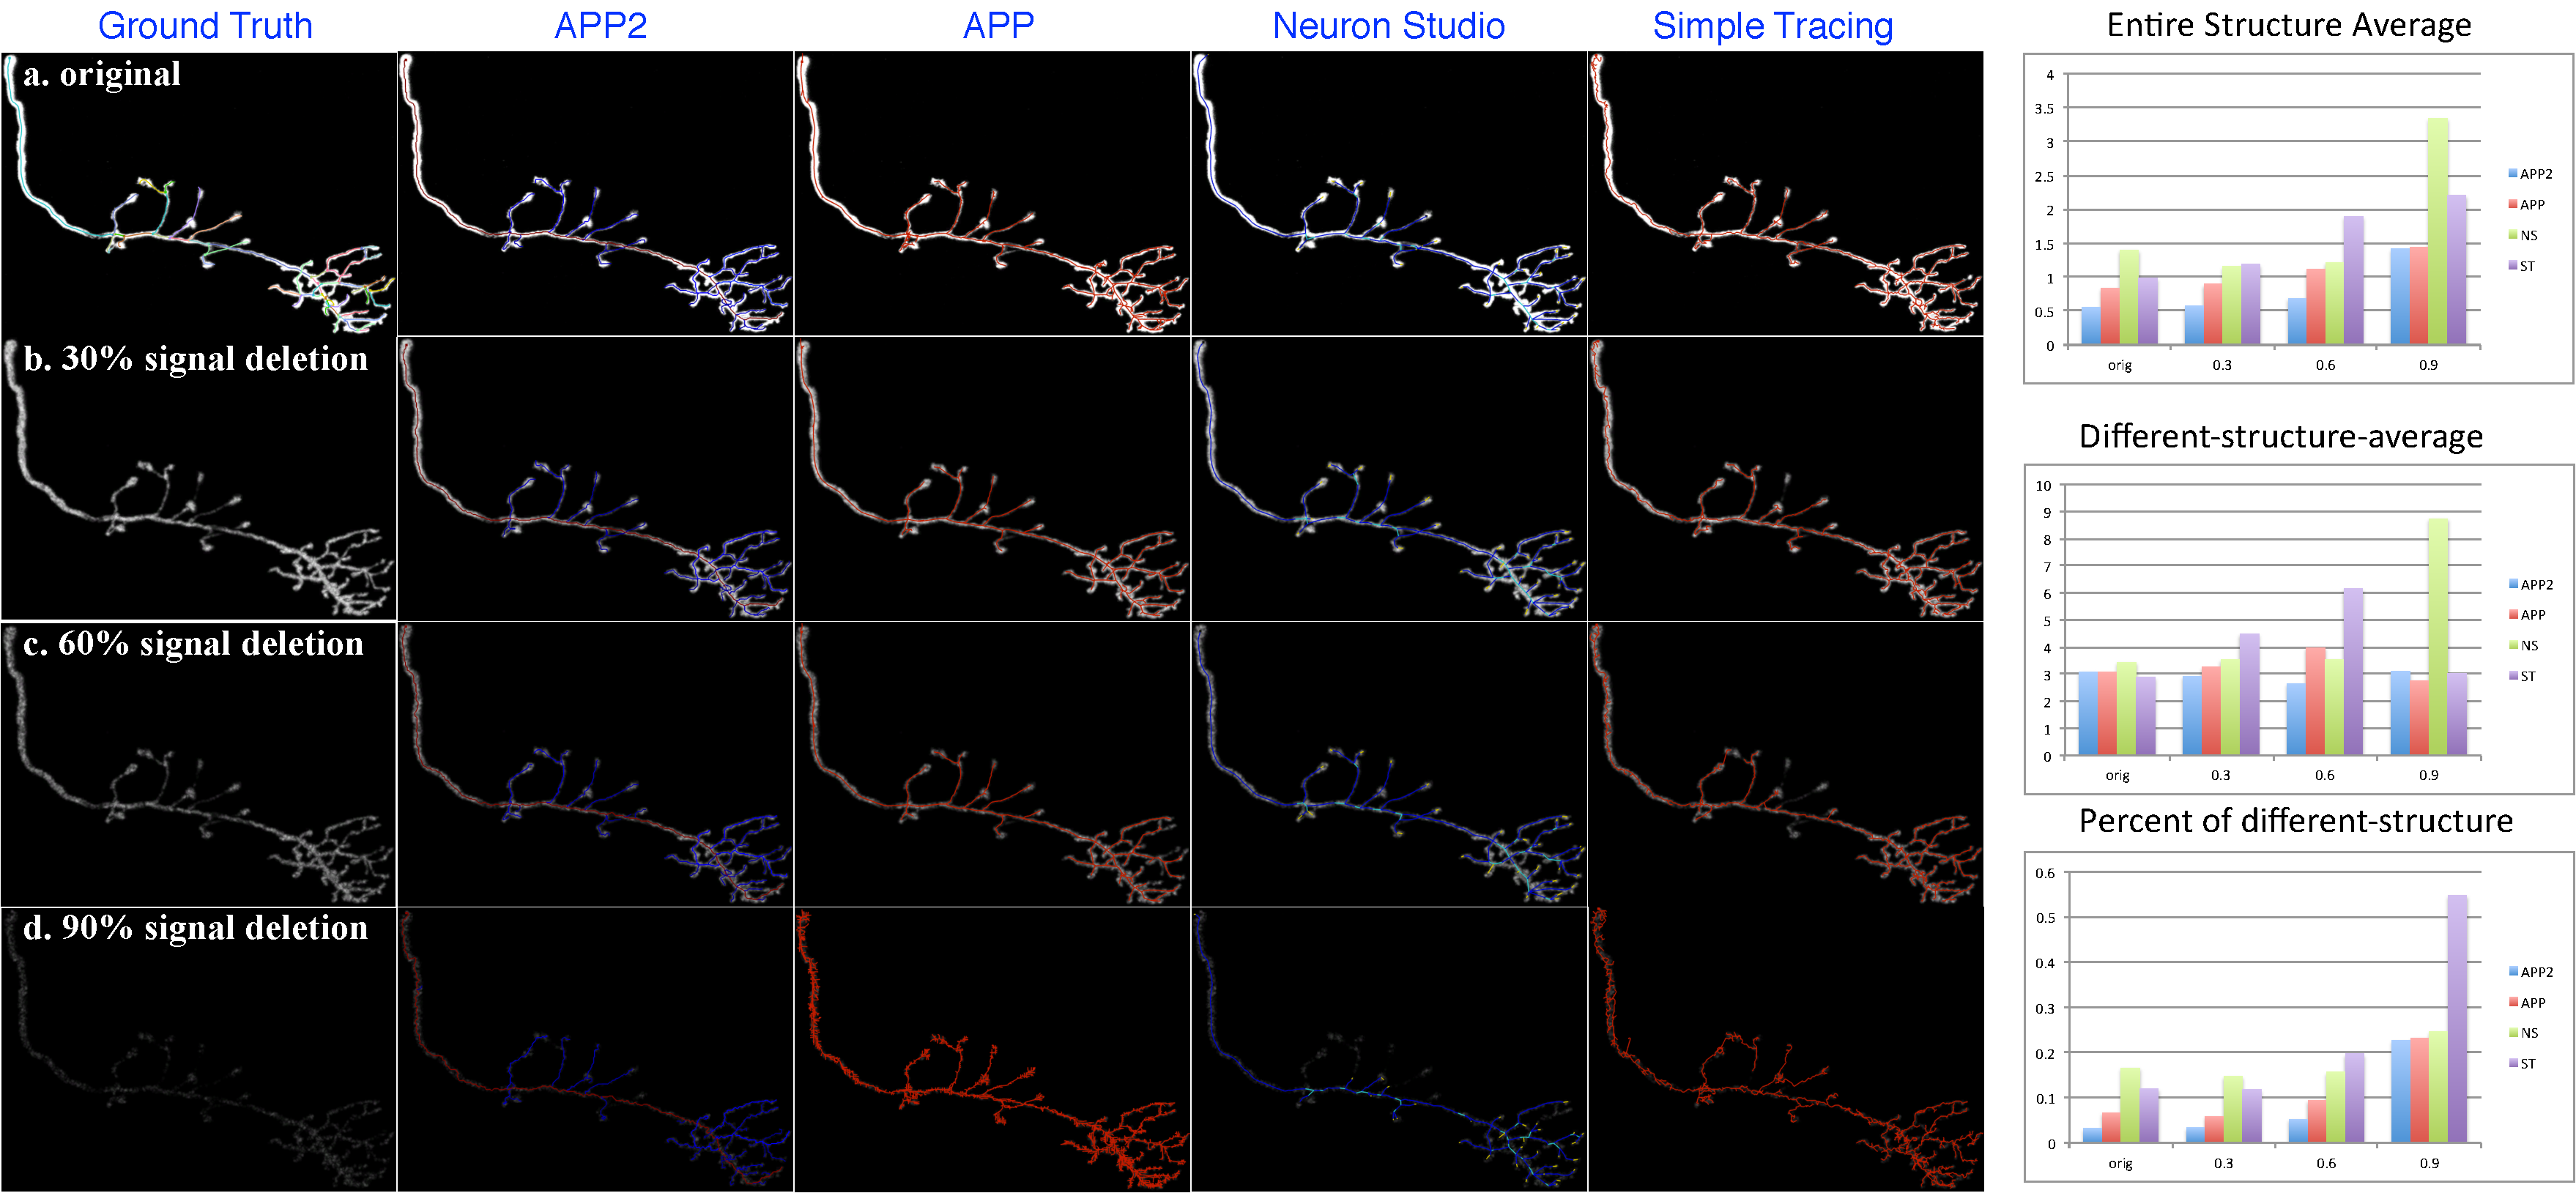
\includegraphics[width=1.0\textwidth]{images/autont_fig3}
\caption[Comparison with different neuron tracing methods subject to the deletion noise]{Comparison with different neuron tracing methods subject to the deletion noise. The reconstructions are overlaid on top of the original images for better visualization. The fourth row corresponds to 90\% signal is deleted. Since it is so dark in this case, we set pixel intensity threshold to 1 so that we are able to compare all different methods. Right side subfigures: the three difference-scores compared to the “ground truth” reconstruction. NS: NeuronStudio. ST: SimpleTracing.}
\label{fig:autont-fig3}
\end{figure}

\begin{figure}[htbp]
\centering
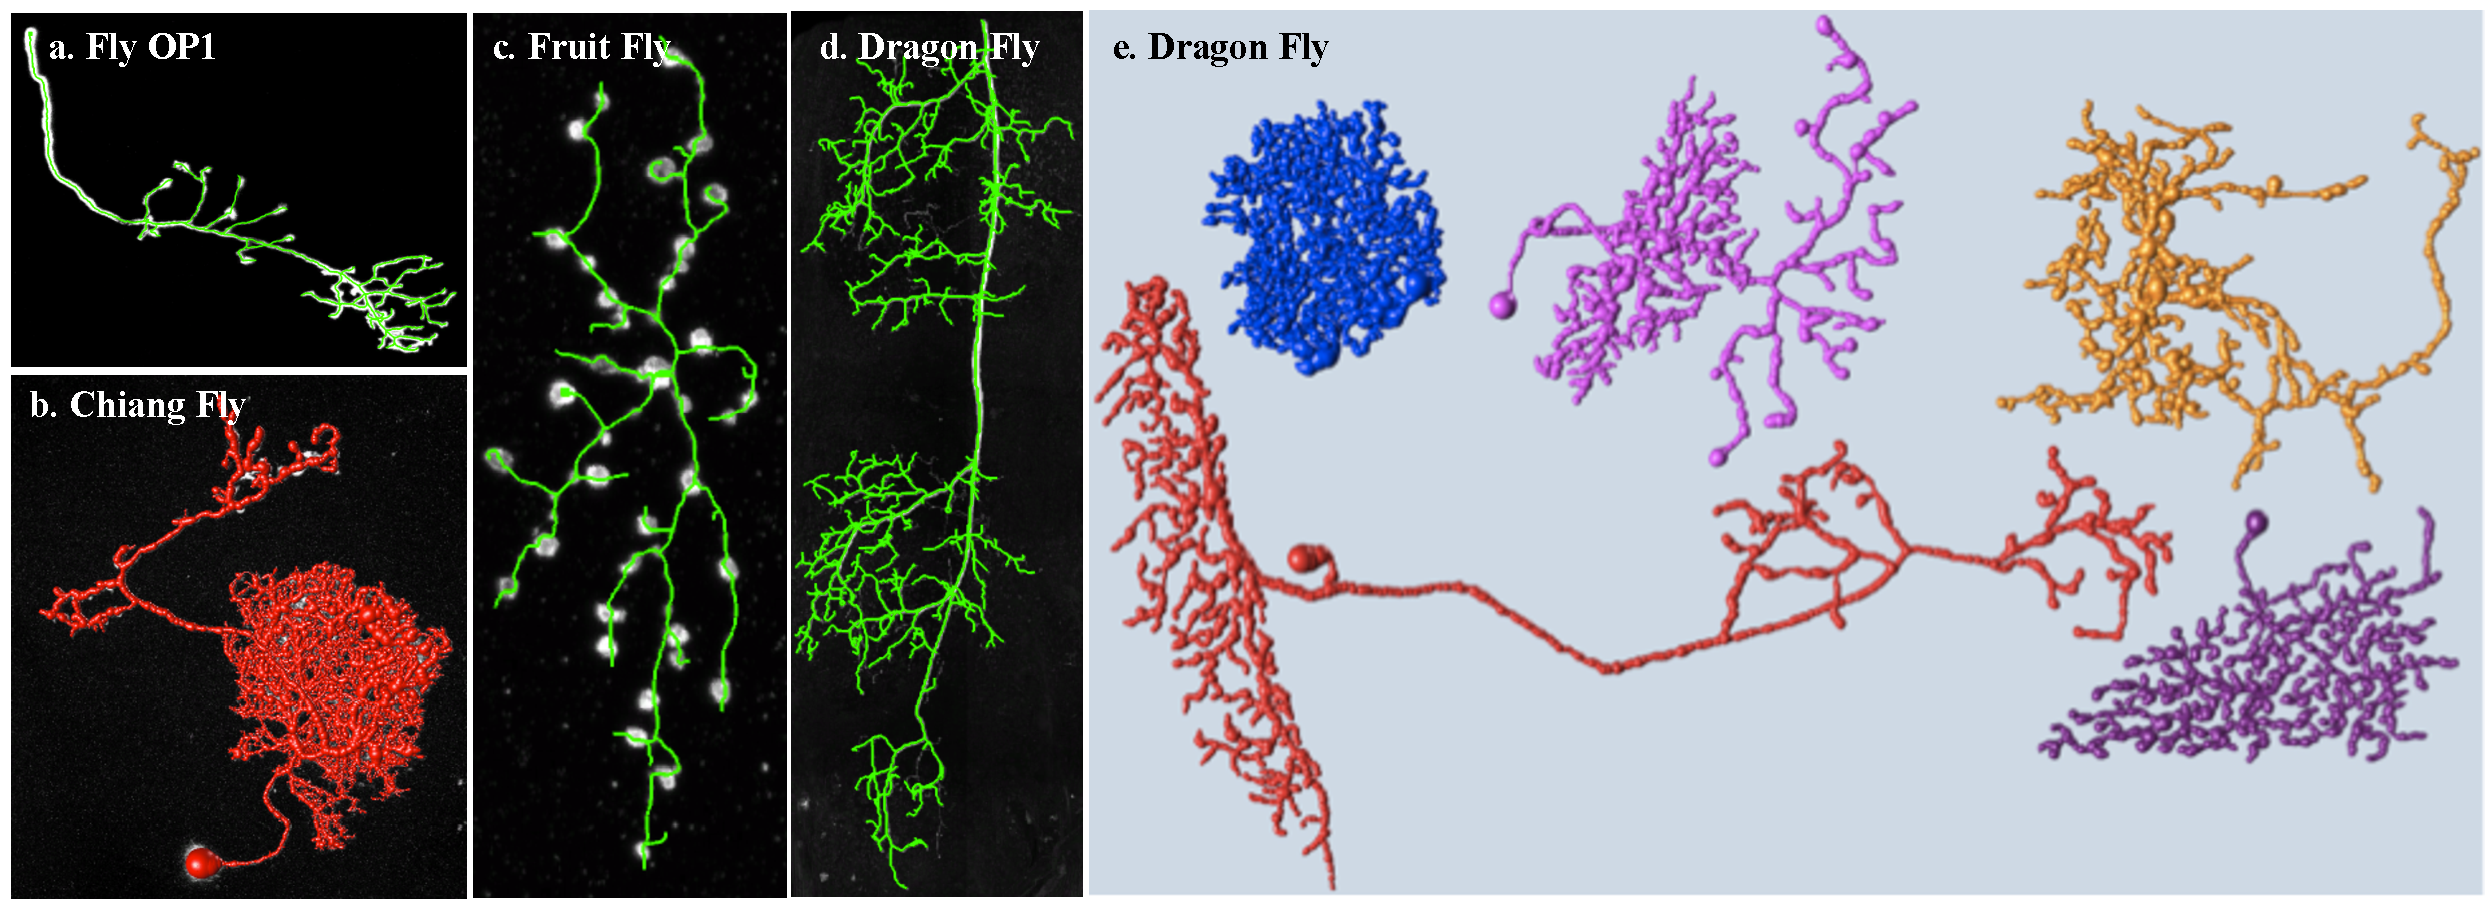
\includegraphics[width=1.0\textwidth]{images/autont_fig4}
\caption[Examples of tracing results on different neuron data sets contributed by different labs]{Examples of tracing results on different neuron data sets contributed by different labs. (a)-(d): tracing results of neurons of different model animals. (e) 3D reconstructed neurons of a large Drosophila neuron image data set with 678 neurons. Different colors indicate different neurons.}
\label{fig:autont-fig4}
\end{figure}

\section{Conclusion}
We present a new neuron-tracing system that contains several nov-el algorithms based on fast marching and hierarchical pruning. We use the fast marching method to compute both the initial neuron reconstruction and the gray-weighted distance transform, and at the same time also improve the robustness of neuron tracing. Hierar-chical pruning sorts the individual segments of an initial recon-struction tree in a hierarchical order, thus facilitates efficient re-moval of redundant segments in the reconstruction. We have com-pared our new method to various previous methods on a number of datasets and found a better performance of the new method in most cases. 

\chapter{Humman guided neuron tracing methods} \label{chpt:manual-nt}
\section{Difficulties for 3D drawing on 2D plane}
\section{Existing methods in Vaa3d}
\section{Fast marching based methods}

\bibliographystyle{plain}
\bibliography{thesis}

\end{document}
